
\section{Per-Metric Evaluation Details}
\label{app:metric_details}

\subsection{Metric Quick Reference}
\label{app:metric_quickref}

\cref{tab:metric_quickref} provides a unified index of all \numsubmetric evaluation sub-metrics. Entries in the \textbf{Detail} column are hyperlinked to the corresponding methodology description.

\begin{table}[H]
\caption[Metric quick-reference]{Metric quick-reference table. ``EM'' = Expert Model; ``VLM'' = vision-language model judge.}
\vspace{+1mm}
\label{tab:metric_quickref}
\centering
\renewcommand{\arraystretch}{1.15}
\scriptsize
\setlength{\tabcolsep}{3pt}
\begin{tabular}{@{}l l l l c@{}}
\toprule
\textbf{Dimension} & \textbf{Sub-Metric} & \textbf{Method} & \textbf{Tool / Model} & \textbf{Detail} \\
\midrule
\multirow{6}{*}{Video Quality}
  & Aesthetic Quality    & EM  & CLIP + LAION head     & \hyperref[app:aesthetic_detail]{\S\ref*{app:aesthetic_detail}} \\
  & Imaging Quality      & EM  & MUSIQ                 & \hyperref[app:imaging_detail]{\S\ref*{app:imaging_detail}} \\
  & Temporal Flickering  & EM  & Pixel MAE             & \hyperref[app:flickering_detail]{\S\ref*{app:flickering_detail}} \\
  & Dynamic Degree       & EM  & RAFT optical flow     & \hyperref[app:dynamic_detail]{\S\ref*{app:dynamic_detail}} \\
  & Motion Smoothness    & EM  & AMT-S interpolation   & \hyperref[app:smoothness_detail]{\S\ref*{app:smoothness_detail}} \\
  & HPSv3-Norm           & EM  & HPSv3                 & \hyperref[app:hps_detail]{\S\ref*{app:hps_detail}} \\
\midrule
\multirow{2}{*}{Setting Adh.}
  & Scene Adherence      & VLM & Doubao-Seed-2.0-lite  & \hyperref[app:scene_adherence_detail]{\S\ref*{app:scene_adherence_detail}} \\
  & Subject Adherence    & VLM & Doubao-Seed-2.0-lite  & \hyperref[app:subject_adherence_detail]{\S\ref*{app:subject_adherence_detail}} \\
\midrule
\multirow{4}{*}{Interaction Adh.}
  & NavScore             & EM  & MegaSaM pose est.     & \hyperref[app:nav_detail]{\S\ref*{app:nav_detail}} \\
  & Event Editing Adh.   & VLM & Doubao-Seed-2.0-lite  & \hyperref[app:event_edit_detail]{\S\ref*{app:event_edit_detail}} \\
  & Subject Action Adh.  & VLM & Doubao-Seed-2.0-lite  & \hyperref[app:subject_action_detail]{\S\ref*{app:subject_action_detail}} \\
  & Persp.\ Switching Adh.  & VLM & Doubao-Seed-2.0-lite  & \hyperref[app:persp_switch_detail]{\S\ref*{app:persp_switch_detail}} \\
\midrule
\multirow{6}{*}{Consistency}
  & Subject Consistency  & EM  & DINOv2 + CLIP + SAM2  & \hyperref[app:subject_consistency_detail]{\S\ref*{app:subject_consistency_detail}} \\
  & Background Cons.     & EM  & CLIP ViT-B/32         & \hyperref[app:background_consistency_detail]{\S\ref*{app:background_consistency_detail}} \\
  & Spatial Consistency  & EM  & MegaSaM + DreamSim    & \hyperref[app:spatial_detail]{\S\ref*{app:spatial_detail}} \\
  & Segment Continuity   & EM  & TransNetV2            & \hyperref[app:segment_continuity_detail]{\S\ref*{app:segment_continuity_detail}} \\
  & Perspective Cons.    & EM  & SAM2   & \hyperref[app:perspective_consistency]{\S\ref*{app:perspective_consistency}} \\
  & Reconstruction Cons. & EM  & Depth Anything 3 reproj. & \hyperref[app:reconstruction_detail]{\S\ref*{app:reconstruction_detail}} \\
\midrule
\multirow{2}{*}{Physical}
  & Causal Fidelity     & VLM & Doubao-Seed-2.0-lite  & \hyperref[app:causal_fidelity_detail]{\S\ref*{app:causal_fidelity_detail}} \\
  & Visual Plausibility & EM & Qwen3VL-35B (ft.)     & \hyperref[app:visual_plausibility_detail]{\S\ref*{app:visual_plausibility_detail}} \\
\bottomrule
\end{tabular}
\end{table}

\tcbset{
  d2box/.style={
    enhanced,
    colback=teal!8,
    colframe=teal!80,
    boxrule=0.5pt,
    arc=3pt,
    left=6pt, right=6pt, top=5pt, bottom=5pt,
    fonttitle=\bfseries\small,
    colbacktitle=teal!35,
    coltitle=black,
    attach boxed title to top left={yshift=-2mm, xshift=4mm},
    boxed title style={arc=2pt, boxrule=0.3pt},
    breakable,
  },
  d3box/.style={
    enhanced,
    colback=orange!8,
    colframe=orange!80,
    boxrule=0.5pt,
    arc=3pt,
    left=6pt, right=6pt, top=5pt, bottom=5pt,
    fonttitle=\bfseries\small,
    colbacktitle=orange!35,
    coltitle=black,
    attach boxed title to top left={yshift=-2mm, xshift=4mm},
    boxed title style={arc=2pt, boxrule=0.3pt},
    breakable,
  },
  d5box/.style={
    enhanced,
    colback=red!8,
    colframe=red!70,
    boxrule=0.5pt,
    arc=3pt,
    left=6pt, right=6pt, top=5pt, bottom=5pt,
    fonttitle=\bfseries\small,
    colbacktitle=red!30,
    coltitle=black,
    attach boxed title to top left={yshift=-2mm, xshift=4mm},
    boxed title style={arc=2pt, boxrule=0.3pt},
    breakable,
  },
  systemprompt/.style={
    colback=gray!10,
    colframe=gray!60,
    boxrule=0.5pt,
    arc=2pt,
    fontupper=\ttfamily\scriptsize,
    left=4pt, right=4pt, top=3pt, bottom=3pt,
    title={\scriptsize\textbf{System Prompt}},
  },
  userprompt/.style={
    colback=blue!8,
    colframe=blue!50,
    boxrule=0.5pt,
    arc=2pt,
    fontupper=\ttfamily\scriptsize,
    left=4pt, right=4pt, top=3pt, bottom=3pt,
    title={\scriptsize\textbf{User Prompt}},
  },
}

This appendix provides per-sub-metric evaluation details organized by dimension. Each sub-metric includes its definition and evaluation examples (VLM prompts or qualitative cases where applicable). The full list of all \numsubmetric sub-metrics is summarized in the unified metric quick-reference table (\cref{tab:metric_quickref} in \cref{app:metric_quickref}).

\subsection{Video Quality}
\label{app:vq_detail}

All six Video Quality sub-metrics are computed by expert models and produce scores in $[0, 100]$ (higher is better).

\subsubsection{Aesthetic Quality}
\label{app:aesthetic_detail}

\myparagraph{Definition.}
Frames are sampled at 2\,FPS. Each frame is encoded by CLIP ViT-L/14, and a LAION Aesthetic linear head~\cite{schuhmann2022laion5b} predicts an aesthetic score in $[0, 10]$. The final score is the mean over all sampled frames, rescaled to $[0, 100]$:
\begin{equation}
  S_{\text{aesth}} = \frac{1}{N}\sum_{i=1}^{N} f_{\text{LAION}}(\text{CLIP}(x_i)) \times 10.
\end{equation}

\subsubsection{Imaging Quality}
\label{app:imaging_detail}

\myparagraph{Definition.}
Frames are sampled at 2\,FPS and resized such that the longer edge $\leq 512$. MUSIQ~\cite{ke2021musiq} predicts a per-frame quality score in $[0, 100]$:
\begin{equation}
  S_{\text{imag}} = \frac{1}{N}\sum_{i=1}^{N} \text{MUSIQ}(x_i).
\end{equation}

\subsubsection{Temporal Flickering}
\label{app:flickering_detail}

\myparagraph{Definition.}
All consecutive frame pairs are compared via pixel-level mean absolute error (MAE). The score is inverted so that lower flickering yields a higher score:
\begin{equation}
  S_{\text{flick}} = \frac{255 - \frac{1}{N-1}\sum_{i=1}^{N-1}\text{MAE}(x_i, x_{i+1})}{255} \times 100.
\end{equation}

\subsubsection{Dynamic Degree}
\label{app:dynamic_detail}

\myparagraph{Definition.}
Frames are sampled at 8\,FPS. RAFT optical flow is computed for each consecutive pair, and the top 5\% magnitude values are averaged per pair:
\begin{equation}
  m_i = \mathrm{mean}\!\bigl(\mathrm{top}_{5\%}\lVert \mathbf{f}_i \rVert\bigr), \quad
  S_{\mathrm{dyn}} =
  \begin{cases}
    100 & \text{if } \sum_{i} \mathbf{1}[m_i > \tau] \geq N_{\min}, \\
    0   & \text{otherwise},
  \end{cases}
\end{equation}
where $\mathbf{f}_i$ is the optical flow field for frame pair $i$, $\tau$ is the dynamic threshold, and $N_{\min}$ is the minimum count of dynamic pairs required.

\subsubsection{Motion Smoothness}
\label{app:smoothness_detail}

\myparagraph{Definition.}
Following VBench, we use AMT-S~\cite{li2023amt} to interpolate even-indexed frames from odd-indexed neighbors, then compute pixel MAE between predicted and actual even frames:
\begin{equation}
  S_{\mathrm{app}} = \frac{255 - \frac{1}{M}\sum_{j=1}^{M}\text{MAE}(\hat{x}_{2j}, x_{2j})}{255} \times 100.
\end{equation}

\subsubsection{HPSv3-Norm}
\label{app:hps_detail}

\myparagraph{Definition.}
We compute the raw HPSv3 reward for each frame and apply linear percentile normalization. Let $p_1$ and $p_{99}$ denote the 1st and 99th percentiles of all per-video mean scores across the evaluated models:
\begin{equation}
  S_{\text{HPS}} = \text{clip}\!\left(\frac{\bar{r} - p_1}{p_{99} - p_1} \times 100,\; 0,\; 100\right),
\end{equation}
where $\bar{r}$ is the per-video mean raw reward. In our evaluation, $p_1 = 5.21$ and $p_{99} = 8.66$.

\subsection{Setting Adherence}
\label{app:setting_detail}

Setting adherence evaluates whether the generated video faithfully realizes the declared world settings.
It comprises two VLM-based sub-metrics: \emph{scene adherence} (environment and offscreen elements) and \emph{subject adherence} (appearance and motion style).
All prompts are issued to \texttt{Doubao-Seed-2.0-lite} with video frames sampled at 2\,fps from the first interaction turn.

\myparagraph{Pre-processing: world-setting decomposition.}
Before evaluation, a VLM automatically decomposes each case's world-setting description into a \emph{visible part} (elements present in the initial frame) and an \emph{offscreen part} (elements expected to appear only after camera movement).
For subject adherence, the subject description is further decomposed into an \emph{appearance part} (visual attributes) and an \emph{action part} (expected movement pattern).
The decomposition is precomputed once per case and shared across all models.

\subsubsection{Scene Adherence}
\label{app:scene_adherence_detail}

\myparagraph{Definition.}
Scene adherence combines two complementary signals:
(i)~\emph{environment maintenance} ($s_{\mathrm{maint}} \in [1,5]$): how well the initially visible scene elements and visual style are preserved across the generated segment;
(ii)~\emph{offscreen content appearance} ($s_{\mathrm{off}} \in \{0,1\}$): whether elements described as offscreen in the initial frame become visible after the prescribed camera movement.
The per-case scene adherence score is $(s_{\mathrm{maint}}/5 + s_{\mathrm{off}}) / 2$.

\myparagraph{Prompt.}
Both aspects are evaluated in a single VLM call with structured JSON output:

\begin{tcolorbox}[d2box, title={Scene Adherence Prompt}]
\ttfamily\scriptsize
You are a video analysis expert. You will see video frames from Turn 1 of a generated video (sampled at 2fps).\\
\\
Evaluate the video on two aspects:\\
\\
**1. Environment Maintenance (1-5)**\\
How well does the video maintain these scene elements that were visible in the initial frame? Also consider whether the visual style remains consistent.\\
Scene description: [VISIBLE\_PART]\\
Visual style: [STYLE]\\
\\
Scoring:\\
- 5: All elements perfectly maintained, style fully consistent\\
- 4: Most elements maintained, style mostly consistent, minor issues\\
- 3: Some elements maintained or style partially drifts\\
- 2: Few elements maintained, significant changes or style mismatch\\
- 1: Scene barely matches the description or style completely wrong\\
\\
**2. Offscreen Content Appearance (0 or 1)**\\
The following elements were described as existing OFF-SCREEN (not visible in the initial frame). Did ANY of them appear in the video as the camera moved?\\
Description: [OFFSCREEN\_PART]\\
\\
- 1: At least one offscreen element appeared\\
- 0: None of the offscreen elements appeared\\
\\
Answer in JSON format ONLY. Each reason must be within 20 words.\\
\{``maintenance'': <1-5>, ``maintenance\_reason'': ``...'', ``offscreen'': <0 or 1>, ``offscreen\_reason'': ``...''\}
\end{tcolorbox}

\subsubsection{Subject Adherence}
\label{app:subject_adherence_detail}

\myparagraph{Definition.}
Subject adherence (third-person cases only) combines:
(i)~\emph{appearance maintenance} ($s_{\mathrm{app}} \in [1,5]$): how well the subject's visual appearance (shape, color, clothing, equipment) is maintained throughout the segment;
(ii)~\emph{action match} ($s_{\mathrm{act}} \in \{0,1\}$): whether the subject exhibits the described movement or action pattern.
The per-case subject adherence score is $(s_{\mathrm{app}}/5 + s_{\mathrm{act}}) / 2$.

\myparagraph{Prompt.}
Both aspects are evaluated in a single VLM call with structured JSON output:

\begin{tcolorbox}[d2box, title={Subject Adherence Prompt}]
\ttfamily\scriptsize
You are a video analysis expert. You will see video frames from Turn 1 of a generated video (sampled at 2fps).\\
\\
Evaluate the video on two aspects:\\
\\
**1. Subject Appearance Maintenance (1-5)**\\
How well does the video maintain the subject's visual appearance (shape, color, clothing, equipment, category)?\\
Subject appearance: [APPEARANCE\_PART]\\
\\
Scoring:\\
- 5: Subject appearance perfectly maintained throughout\\
- 4: Mostly maintained, minor visual changes\\
- 3: Some features maintained, noticeable changes\\
- 2: Few features maintained, significant appearance drift\\
- 1: Subject barely recognizable or completely changed\\
\\
**2. Subject Action (0 or 1)**\\
Does the subject exhibit the described movement/action pattern in the video?\\
Expected action: [ACTION\_PART]\\
\\
- 1: The described action/movement pattern is clearly visible\\
- 0: The action/movement pattern is not visible or completely different\\
\\
Answer in JSON format ONLY. Each reason must be within 20 words.\\
\{``maintenance'': <1-5>, ``maintenance\_reason'': ``...'', ``action'': <0 or 1>, ``action\_reason'': ``...''\}
\end{tcolorbox}

\subsection{Interaction Adherence}
\label{app:interaction_detail}

Interaction adherence comprises navigation trajectory evaluation (expert model) and three VLM-based sub-metrics for event editing, subject action, and perspective switching.

\subsubsection{NavScore}
\label{app:nav_detail}

\myparagraph{Definition.}
NavScore evaluates navigation accuracy by comparing predicted camera trajectories against synthetic ground-truth (GT) trajectories constructed from the action sequence.

\myparagraph{Camera pose estimation.}
We extract per-frame camera-to-world poses using MegaSaM~\cite{li2024megasam}, a monocular structure-from-motion method that produces dense 4$\times$4 pose matrices from video.
Each multi-turn video yields a single globally consistent pose sequence, which is then split at turn boundaries for per-turn and global analysis.

\myparagraph{Ground-truth trajectory construction.}
GT trajectories are built adaptively per turn based on the action type:
\begin{itemize}[leftmargin=1.5em, nosep]
  \item \emph{Pure translation} (W/S/A/D): a straight-line trajectory in the action direction under the initial camera orientation, with length matched to the predicted displacement. If the predicted displacement is below a minimum threshold ($0.1$ units), a fallback length of $1.0$ is used to penalize non-responsive models.
  \item \emph{Rotation} (left/right/up/down): an adaptive orbital trajectory with radius $R$ and angle $\theta$ estimated from the predicted trajectory via $R = \text{chord} / (2\sin(\theta/2))$. For third-person perspectives, $R$ has a minimum of $1.0$ to prevent degenerate orbits. If the predicted rotation is below $3^\circ$, fallback parameters ($\theta = 30^\circ$, $R = 1.0$) are applied.
\end{itemize}
The GT is then aligned to the predicted coordinate frame (translation offset + rotation alignment), while the predicted trajectory remains unchanged.

\myparagraph{Arc-length resampling.}
To ensure equal weighting across turns regardless of frame count or motion speed, both GT and predicted trajectories are resampled to a fixed number of points ($K = 20$) uniformly along their respective arc lengths.
Position is linearly interpolated and rotation is interpolated via Slerp along the arc-length parameter.

\myparagraph{Evaluation metrics.}
We evaluate navigation accuracy using normalized Absolute Trajectory Error (ATE), which measures the global shape agreement between predicted and ground-truth trajectories after per-turn arc-length resampling and concatenation:
\begin{align}
  \mathrm{nATE}_t &= \min\!\left(\frac{\mathrm{ATE}_t}{\max(L_{\mathrm{pred}},\; 0.5)},\; 1\right), \label{eq:nate_t} \\
  \mathrm{nATE}_r &= \min\!\left(\frac{\mathrm{ATE}_r}{\max(\Theta_{\mathrm{pred}},\; 10^\circ)},\; 1\right),
\end{align}
where $L_{\mathrm{pred}}$ and $\Theta_{\mathrm{pred}}$ are the predicted path length and total rotation.
The minimum denominators ($0.5$ for translation, $10^\circ$ for rotation) prevent instability when the model produces near-zero motion.
We also compute Relative Pose Error (RPE) and report it as an auxiliary diagnostic, but it is excluded from the final score because action-conditioned world models often exhibit non-uniform motion profiles, making frame-level velocity-matched GT trajectories unreliable.
ATE therefore serves as the primary signal for trajectory-shape correctness.

\myparagraph{Trajectory consistency.}
For repeated or symmetric actions, we compare all valid same-group turn pairs, including W$\leftrightarrow$S, A$\leftrightarrow$D, left$\leftrightarrow$right, and up$\leftrightarrow$down.
Each turn is first normalized to its own start pose, and symmetric pairs are mirrored into a shared canonical frame when needed.
We then compute pairwise normalized ATE between the two turns and average over all valid pairs:
\begin{align}
  \mathrm{cnATE}_t &= \frac{1}{P}\sum_{p=1}^{P} \mathrm{nATE}^{(p)}_t, \\
  \mathrm{cnATE}_r &= \frac{1}{P}\sum_{p=1}^{P} \mathrm{nATE}^{(p)}_r,
\end{align}
where $P$ is the number of valid same-group turn pairs.
The trajectory consistency term is then defined as
\begin{equation}
  \mathrm{Cons} = 1 - \frac{\mathrm{cnATE}_t + \mathrm{cnATE}_r}{2}.
\end{equation}
If no valid same-group pair exists, we set $\mathrm{cnATE}_t = \mathrm{cnATE}_r = 0$, which yields $\mathrm{Cons} = 1$.

\myparagraph{NavScore aggregation.}
The final NavScore for each video is computed as
\begin{align}
  \mathrm{Acc} &= 1 - \frac{\mathrm{nATE}_t + \mathrm{nATE}_r}{2}, \\
  \mathrm{NavScore} &= \frac{\mathrm{Acc} + \mathrm{Cons}}{2}.
\end{align}
Model-level scores are the mean across all navigation cases, rescaled to $[0, 100]$.

\myparagraph{Qualitative Results.}
\cref{fig:navi_visualize} shows a four-turn navigation case (T1: \texttt{W}, T2: $\rightarrow$, T3: $\rightarrow$, T4: $\leftarrow$) evaluated on three models. Happy Oyster and HY-World~1.5 produce trajectories that consistently follow the instructed directions across all turns, while HY-Video~1.5 reverses the rotation direction in T2 and T3, resulting in clear trajectory deviation.
\cref{fig:7panels_gt_pred} illustrates how the adaptive ground-truth is constructed per model. Because different models accept different input interfaces and exhibit varying motion magnitudes, the GT trajectory adapts its scale to the predicted path length. Both Happy Oyster and HY-World~1.5 navigate correctly but with different amplitudes, so their adaptive GTs differ in scale while both yielding high NavScores. In contrast, HY-Video~1.5 moves in the wrong direction, and the adaptive GT faithfully reflects this directional error, penalizing it appropriately.

\begin{figure}[H]
\centering
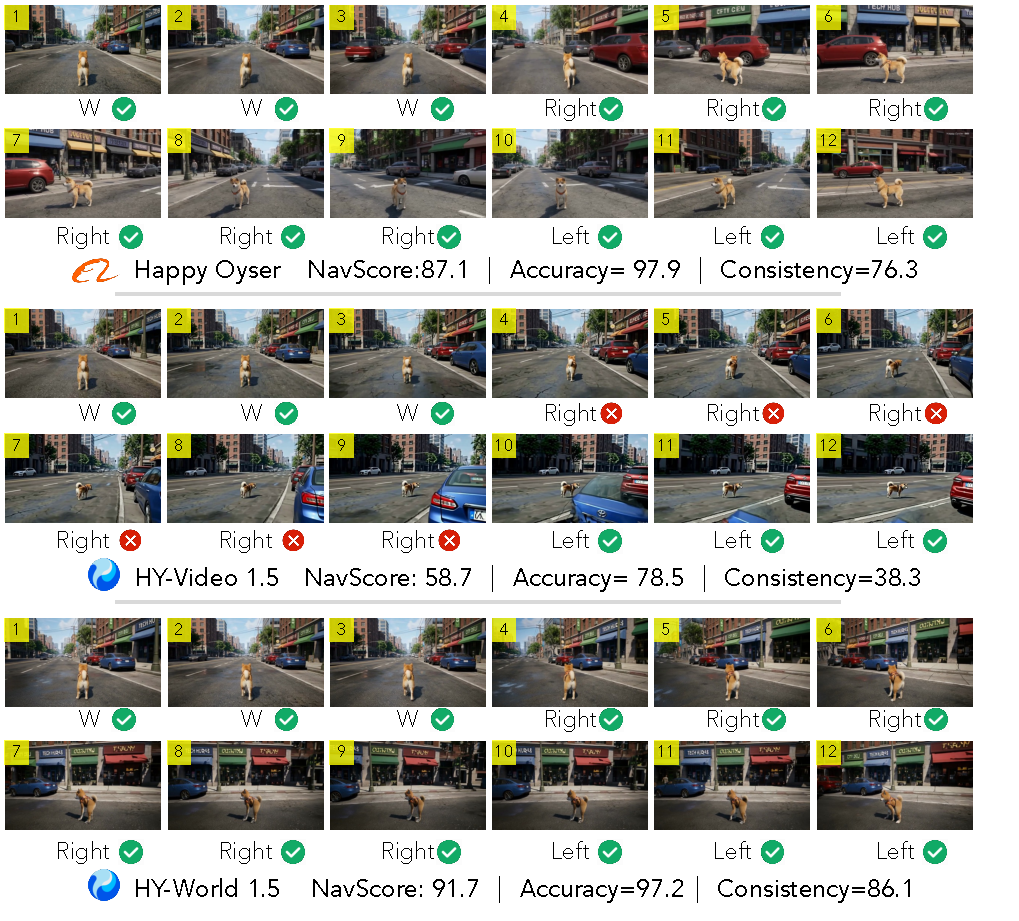
\includegraphics[width=\linewidth]{figures/appendix/navi_visualize.pdf}
\caption[Navigation qualitative comparison]{A four-turn navigation case (T1: \texttt{W}, T2: $\rightarrow$, T3: $\rightarrow$, T4: $\leftarrow$) across three models. Frames 1--3 correspond to T1, 4--6 to T2, 7--9 to T3, and 10--12 to T4. Happy Oyster and HY-World~1.5 follow the instructed directions correctly, while HY-Video~1.5 reverses the rotation in T2 and T3.}
\label{fig:navi_visualize}
\end{figure}

\begin{figure}[H]
\centering
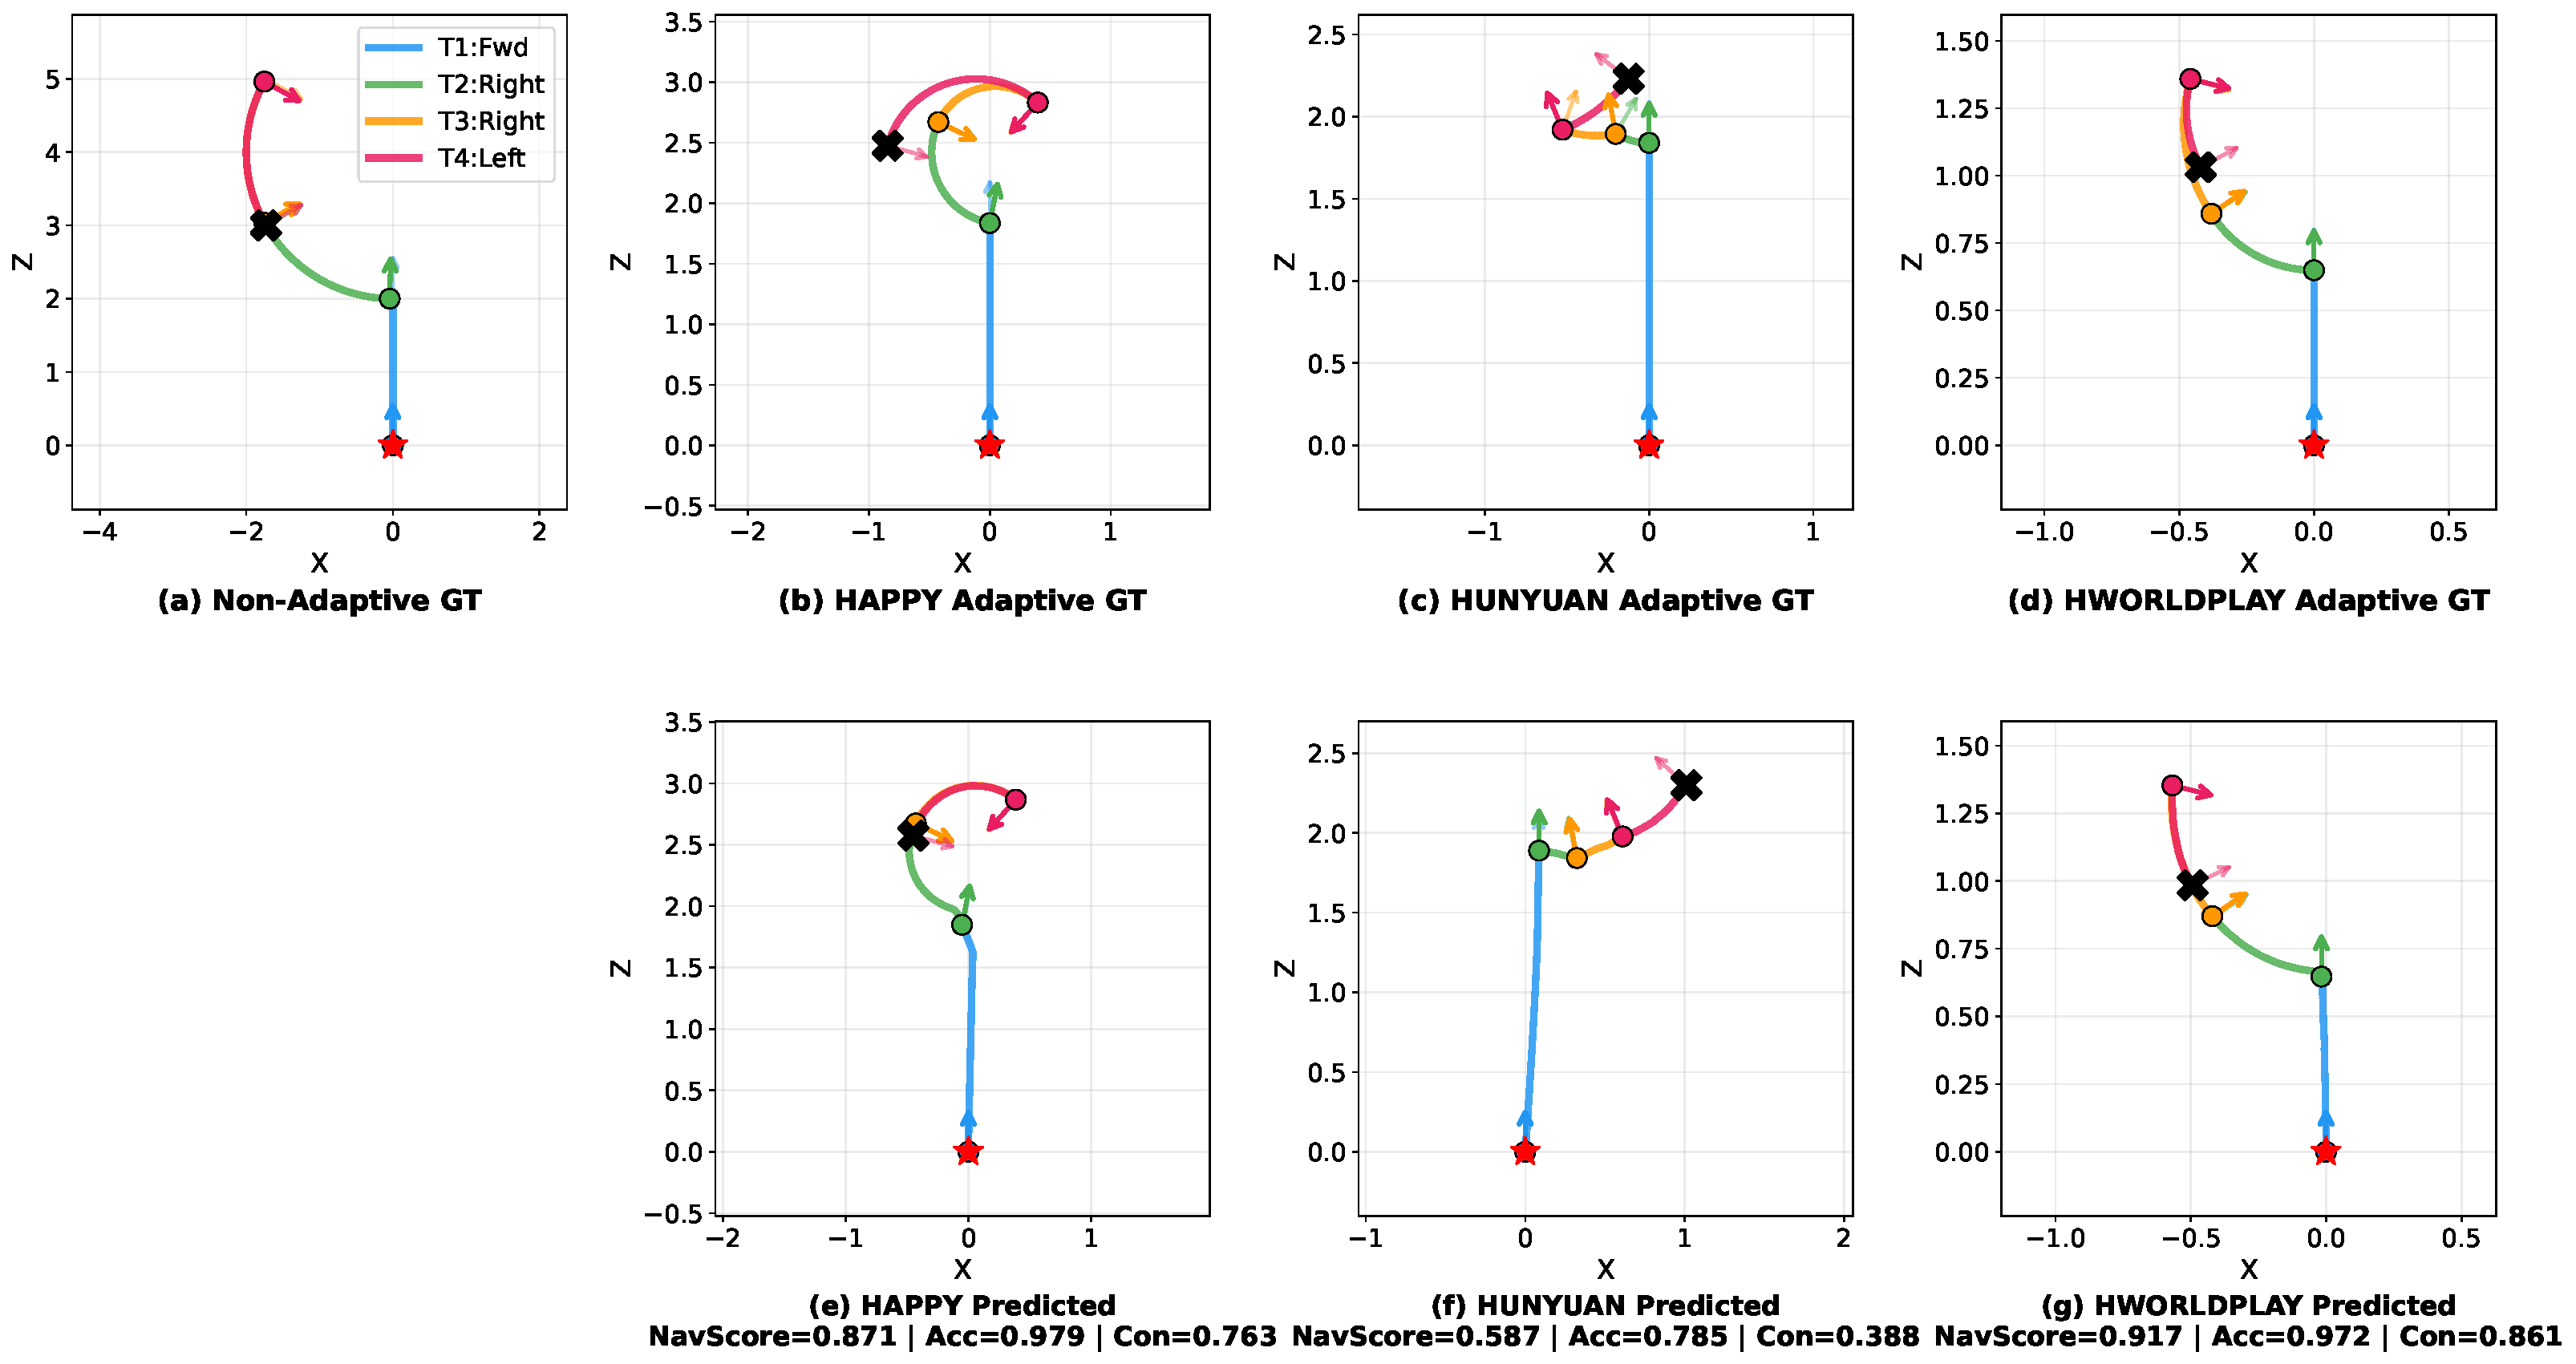
\includegraphics[width=\linewidth]{figures/appendix/7panels_gt_pred.pdf}
\caption[Adaptive ground-truth construction]{Adaptive GT construction for the same case. The GT trajectory adapts to each model's predicted motion magnitude, so correctly navigating models with different amplitudes (Happy Oyster vs.\ HY-World~1.5) both receive fair evaluation. For HY-Video~1.5, the wrong-direction motion is captured as trajectory error rather than a scale mismatch.}
\label{fig:7panels_gt_pred}
\end{figure}

\subsubsection{Event Editing Adherence}
\label{app:event_edit_detail}

\myparagraph{Definition.}
Event editing adherence uses \texttt{Doubao-Seed-2.0-lite} with video frames sampled at 3\,fps. Five progressive binary questions are asked per turn, each with an \emph{expected} answer. The turn receives one point per question whose response matches the expected answer, yielding a raw score in $[0,5]$. The case score is the mean over all event-edit turns, rescaled to $[0, 100]$ by multiplying by $20$.

\myparagraph{Prompt.}
Event editing and subject action share the following system prompt:

\begin{tcolorbox}[d3box, title={Shared System Prompt (event editing \& subject action)}]
\begin{tcolorbox}[systemprompt]
You are evaluating AI-generated video segments from interactive world models. Each video segment corresponds to one interaction turn where a specific event was instructed to happen.\\
\\
Your task: answer with ONLY `Yes' or `No' based on what you observe in the provided frames. Follow these guidelines:\\
- These are AI-generated videos, not real footage. Minor visual artifacts, slight inconsistencies, or imperfect rendering should NOT cause a `No' if the overall intent is recognizable.\\
- Focus on whether the CORE semantic meaning of the described event is visually present, not whether every literal detail matches perfectly.\\
- A long or detailed event description may only be partially depicted. Judge based on whether the main action or change is recognizable.\\
- When in doubt between Yes and No, lean toward the interpretation that better matches what you actually see, not what you expect to see.
\end{tcolorbox}
\vspace{2pt}
\textit{\small Each response is followed by a one-line \texttt{Reason:} field (at most 50 words) that names the specific issue whenever the point is not awarded.}
\end{tcolorbox}

\vspace{6pt}

\begin{tcolorbox}[d3box, title={Event Editing Adherence (Q1--Q5)}]
\ttfamily\scriptsize
World setting: [SCENE\_DESCRIPTION]\\
Interaction instruction for this turn: [ACTION]\\
\\
The following frames are uniformly sampled from the generated video segment for this turn.\\
\mbox{[FRAME\_SEQUENCE]}\\
\\
Q1 (Static Scene Check): Does the scene remain largely unchanged, with no clear indication of `[ACTION]' occurring? \emph{Answer No if there is ANY recognizable change related to this event.} Expected: \texttt{No}.\\
Q2 (Event Occurrence): Does the video show something resembling or consistent with the described event `[ACTION]'? \emph{Partial depiction counts as Yes.} Expected: \texttt{Yes}.\\
Q3 (Event Completion): By the end of this segment, has the described event `[ACTION]' reached a clear conclusion or outcome? \emph{Ongoing events without a visible end state receive No.} Expected: \texttt{Yes}.\\
Q4 (Detail Accuracy): Are the key details of `[ACTION]' accurately depicted, such as the correct objects, agents, directions, and quantities? Expected: \texttt{Yes}.\\
Q5 (Anomaly Absence): Does any unexpected object, entity, or visual anomaly unrelated to `[ACTION]' appear in this segment? \emph{Natural consequences of the event and minor AI rendering artifacts do not count.} Expected: \texttt{No}.
\end{tcolorbox}

\myparagraph{Qualitative Results.}
\cref{fig:qual_ee} contrasts representative outputs across models on two event-edit turns. High-scoring cases exhibit a clear state transition aligned with the instructed event (matching Q2--Q3), while low-scoring cases either leave the scene untouched (Q1 fires) or introduce unrelated entities that trigger the anomaly check (Q5).

\begin{figure}[H]
\centering
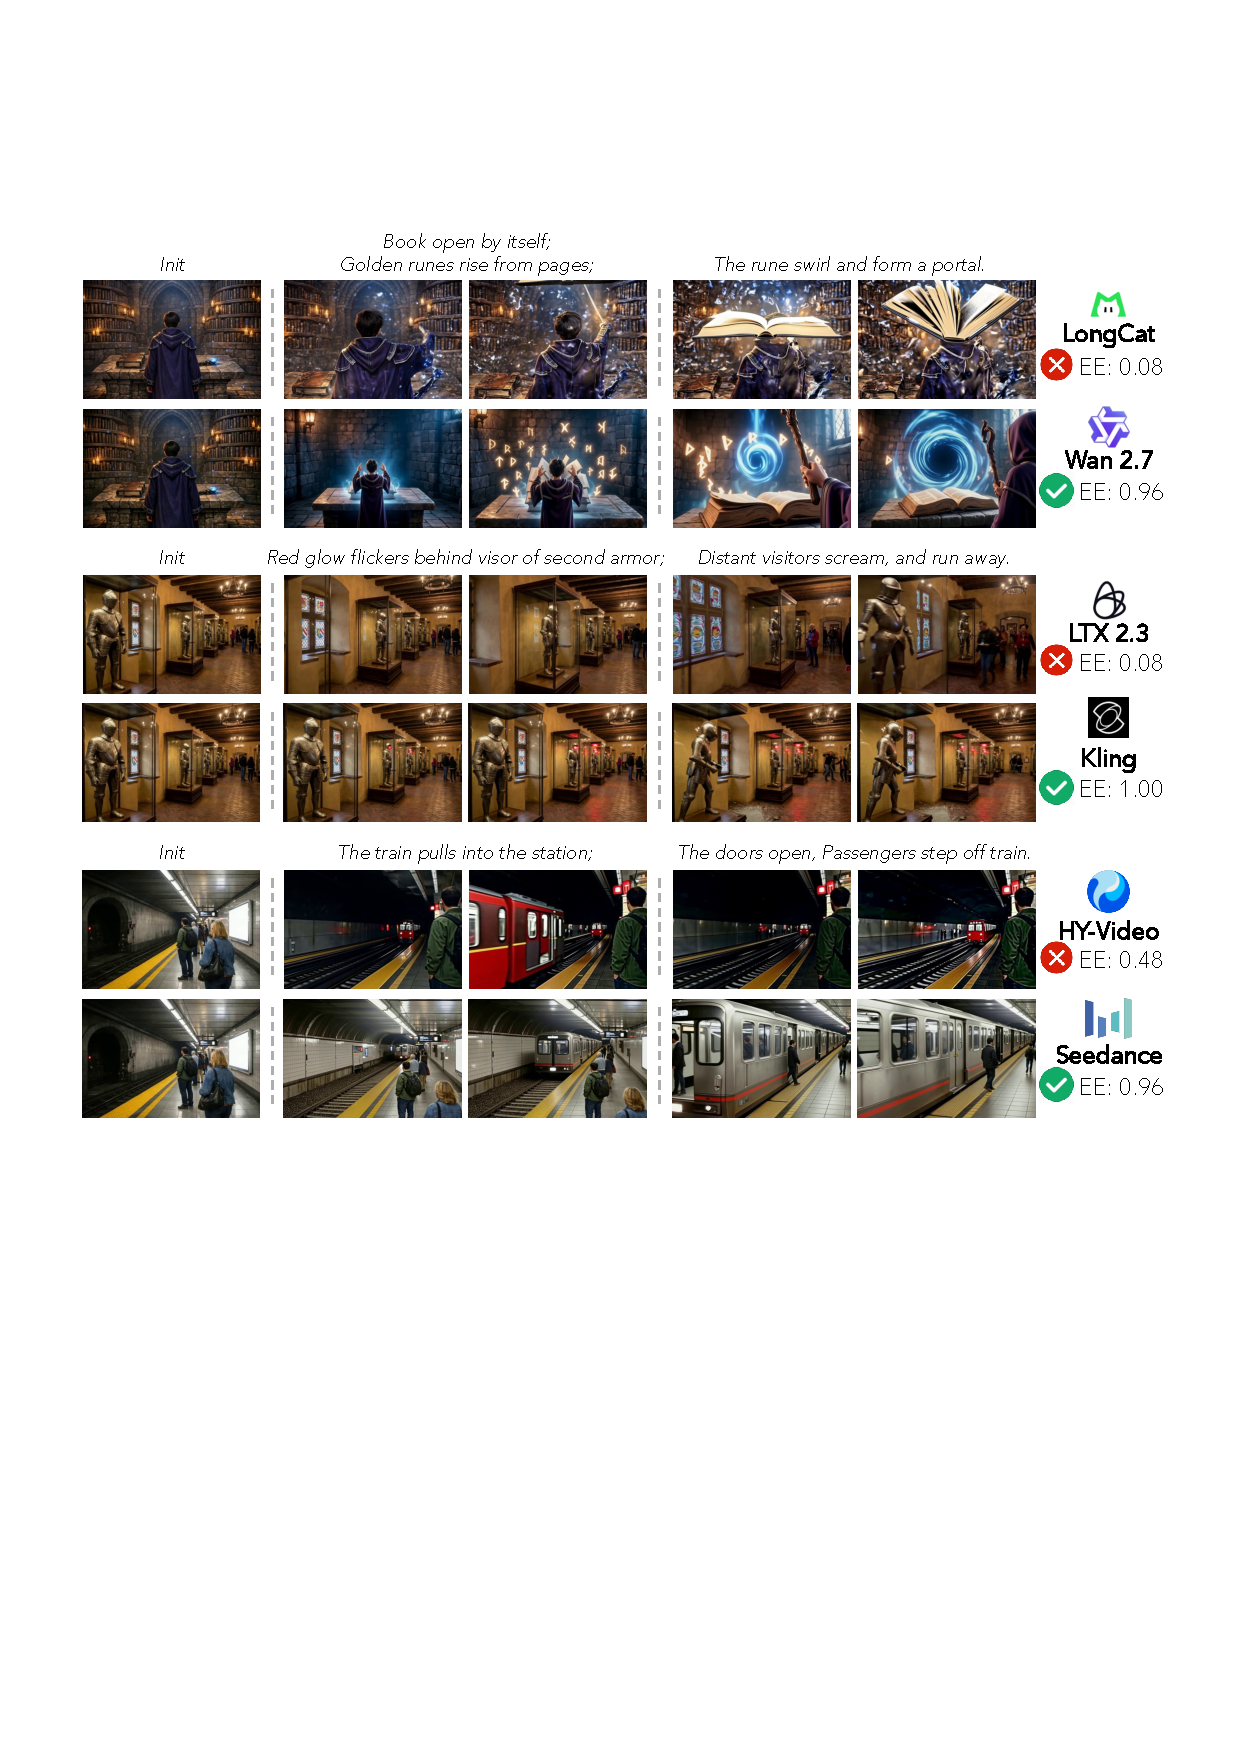
\includegraphics[width=\linewidth]{figures/EE_case.orig.pdf}
\caption[Qualitative comparisons on event editing]{Qualitative comparisons on event editing.}
\label{fig:qual_ee}
\end{figure}

\subsubsection{Subject Action Adherence}
\label{app:subject_action_detail}

\myparagraph{Definition.}
Subject action adherence uses the same shared system prompt and five-question scoring rule as event editing adherence, but with question templates tuned to whether the subject performs the instructed action. The case score is the mean over all subject-action turns.

\myparagraph{Prompt.} We show the prompt below.

\begin{tcolorbox}[d3box, title={Subject Action Adherence (Q1--Q5)}]
\ttfamily\scriptsize
World setting: [SCENE\_DESCRIPTION]\\
Interaction instruction for this turn: [ACTION]\\
\\
The following frames are uniformly sampled from the generated video segment for this turn.\\
\mbox{[FRAME\_SEQUENCE]}\\
\\
Q1 (Idle Subject Check): Does the subject remain idle or stationary, with no attempt to perform `[ACTION]'? \emph{Answer No if the subject shows ANY movement or gesture related to this action.} Expected: \texttt{No}.\\
Q2 (Action Occurrence): Does the video show the subject performing something resembling or consistent with `[ACTION]'? \emph{Partial execution counts as Yes.} Expected: \texttt{Yes}.\\
Q3 (Action Completion): By the end of this segment, has the subject's action `[ACTION]' reached a clear conclusion or outcome? Expected: \texttt{Yes}.\\
Q4 (Detail Accuracy): Are the key details of `[ACTION]' accurately depicted, such as the correct subject, target objects, and manner of the action? Expected: \texttt{Yes}.\\
Q5 (Unnatural Motion Check): Does the subject exhibit any unnatural body movement, impossible pose, or physically implausible interaction while performing `[ACTION]'? \emph{Only clearly unnatural movements or impossible poses count; slight jitter or minor hand artifacts do not.} Expected: \texttt{No}.
\end{tcolorbox}

\myparagraph{Qualitative Results.}
\cref{fig:qual_sa} illustrates how subject-action adherence differentiates models on the same instruction. Successful generations show the subject initiating and completing the prescribed action successfully, whereas failure cases leave the subject idle or execute only a partial gesture that never reaches a clear end state.

\begin{figure}[H]
\centering
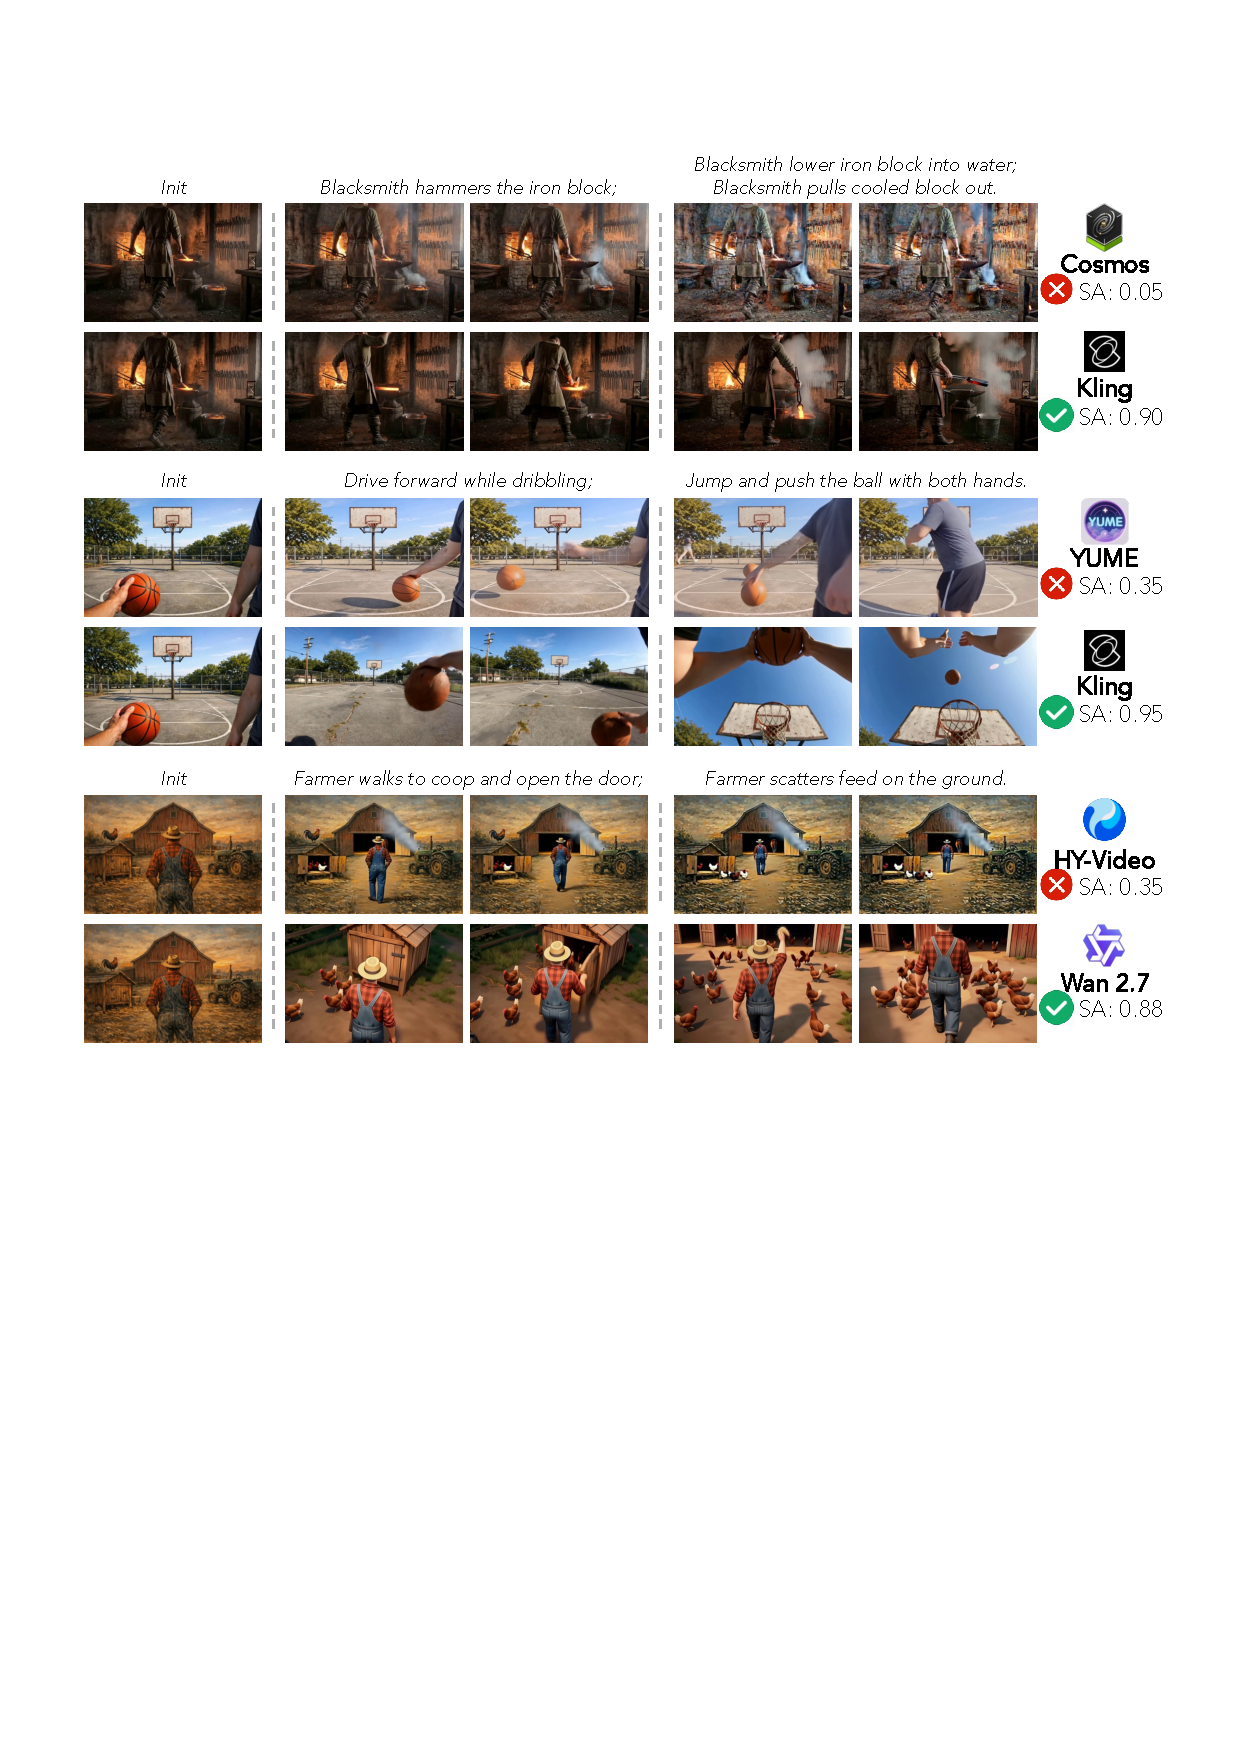
\includegraphics[width=\linewidth]{figures/SA_case.orig.pdf}
\caption[Qualitative comparisons on subject action]{Qualitative comparisons on subject action.}
\label{fig:qual_sa}
\end{figure}

\subsubsection{Perspective Switching Adherence}
\label{app:persp_switch_detail}

\myparagraph{Definition.}
Perspective switching adherence evaluates whether the model can transition between first-person and third-person views. Three binary questions are asked per turn. A turn receives a score of 1 only if all three answers are \texttt{Yes} ($Q1 \wedge Q2 \wedge Q3$), and 0 otherwise.

\myparagraph{Prompt.} We provide the prompt below. We provide the prompt below.

\begin{tcolorbox}[d3box, title={Perspective Switching Adherence (Q1--Q3)}]
\textbf{System:}
\begin{tcolorbox}[systemprompt]
You are a precise video evaluator. You will be given frames from the beginning and end of a generated video turn and a perspective-switching instruction. Answer each question with Yes or No only.
\end{tcolorbox}
\vspace{4pt}
\textbf{User:}
\begin{tcolorbox}[userprompt]
Perspective switching instruction: [SWITCH\_INSTRUCTION]\\
(e.g., ``Switch from first-person to third-person view following the character'')\\
Source perspective: [SOURCE\_PERSPECTIVE] (first-person / third-person)\\
Target perspective: [TARGET\_PERSPECTIVE] (first-person / third-person)\\
\\
Early frames (beginning of the turn segment):\\
\mbox{[EARLY\_FRAME\_SEQUENCE]}\\
Late frames (end of the turn segment):\\
\mbox{[LATE\_FRAME\_SEQUENCE]}\\
\\
Answer each question with Yes or No only.\\
\\
Q1 (Transition Visibility): Can a clear change in perspective be observed between the early and late frames?\\
Q2 (Target Consistency): Does the late-frame perspective match the target perspective ([TARGET\_PERSPECTIVE])?\\
Q3 (Quality Compliance): Does the new perspective satisfy expected structural properties? For third-person, is the subject centered with a following camera? For first-person, are there no self-view artifacts?
\end{tcolorbox}
\end{tcolorbox}

\myparagraph{Qualitative Results.}
\cref{fig:qual_ps} shows some text-driven model cases on the same switching instruction. Successful cases satisfy all three checks with a clear perspective change, a scene matching, and a structurally clean framing, while failures either preserve the source perspective.

\begin{figure}[H]
\centering
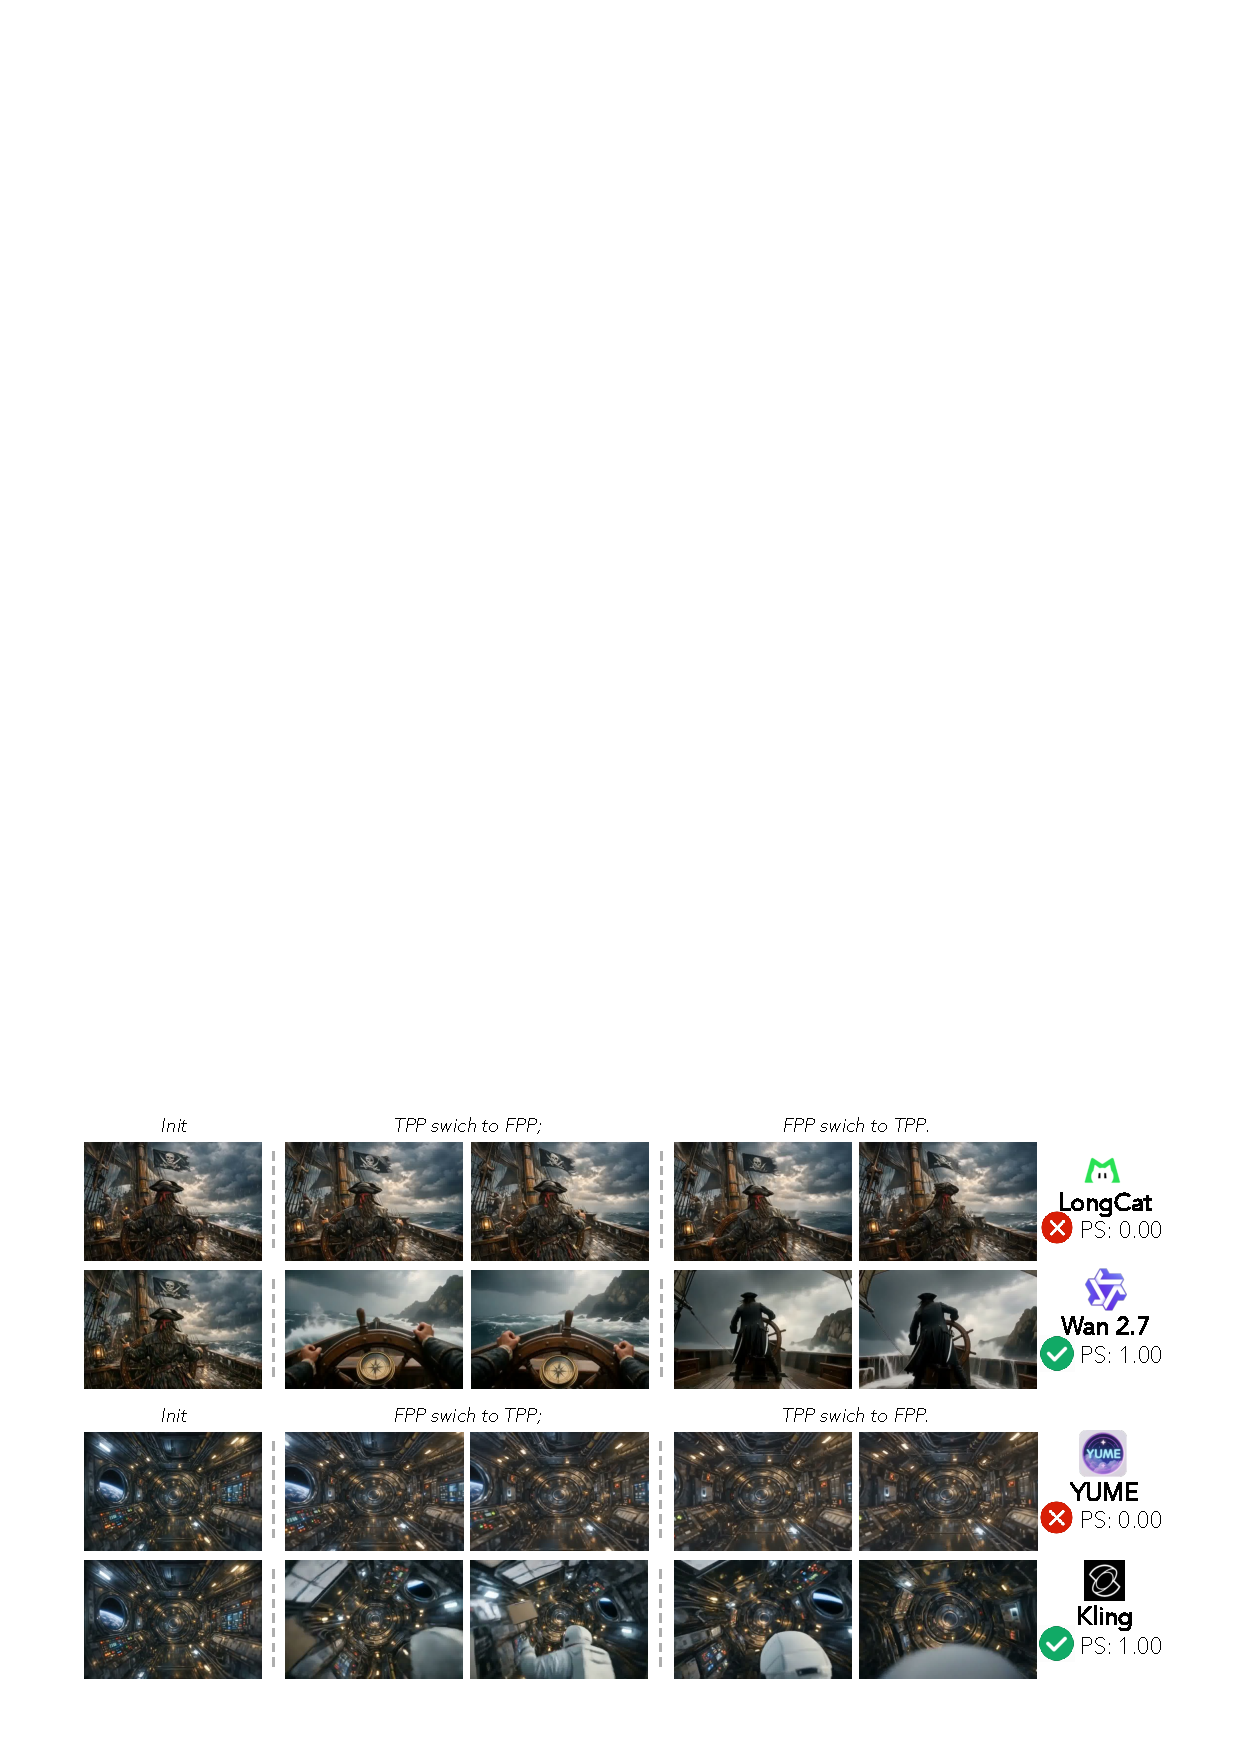
\includegraphics[width=\linewidth]{figures/PS_case.orig.pdf}
\caption[Qualitative comparisons on perspective switching]{Qualitative comparisons on perspective switching.}
\label{fig:qual_ps}
\end{figure}

\subsection{Consistency}
\label{app:consistency_details}

All seven consistency sub-metrics measure frame-level temporal coherence within each generated clip.

\subsubsection{Subject Consistency}
\label{app:subject_consistency_detail}

\myparagraph{Definition.}
For each frame with a valid SAM2 mask (area $\geq 10$\,px), we crop the subject region (background filled with gray) and extract DINOv2 ViT-B/14 and CLIP ViT-B/16 features.
We compute two similarity signals:
(i) DINOv2 adjacent-frame cosine similarity $s_i^{\mathrm{dino}} = \cos(\mathbf{f}_{i-1}, \mathbf{f}_i)$, and
(ii) CLIP first-frame anchored similarity $s_i^{\mathrm{clip}} = \cos(\mathbf{f}_0, \mathbf{f}_i)$.
The per-frame score is $(s_i^{\mathrm{dino}} + s_i^{\mathrm{clip}})/2$, averaged across all valid frames.

\subsubsection{Background Consistency}
\label{app:background_consistency_detail}

\myparagraph{Definition.}
Following VBench, we extract CLIP ViT-B/32 features from each frame and compute the mean cosine similarity between consecutive frame pairs: $\mathrm{score} = \frac{1}{N-1}\sum_{i=1}^{N-1} \cos(\mathbf{f}_i, \mathbf{f}_{i+1})$.

\subsubsection{Spatial Consistency}
\label{app:spatial_detail}

\myparagraph{Definition.}
For roundtrip trajectories, we use MegaSaM-estimated camera poses to identify the \emph{return frame} in the final turn, i.e., the frame whose rotation matrix $R_k$ minimizes $\arccos\!\bigl((\mathrm{tr}(R_0^\top R_k) - 1)/2\bigr)$ relative to the first frame.
Let $s_{\mathrm{ret}}$ be the DreamSim similarity between the first frame and this return frame, computed as $1/(1+d)$ where $d$ is the DreamSim distance.
We uniformly sample 10 intermediate frames and compute the minimum similarity $s_{\mathrm{min}}$ to the first frame.
A motion gate prevents trivially high scores from near-static videos:
\begin{equation}
  \mathrm{score} = s_{\mathrm{ret}} \cdot \min\!\Bigl(1,\; \frac{1 - s_{\mathrm{min}}}{\tau}\Bigr), \quad \tau = 0.15.
\end{equation}
\myparagraph{Qualitative Results.}
\cref{fig:qual_spatial} illustrates the motion gate at work. The near-static return frame genereted by LongCat-Video earns a high $s_{\mathrm{ret}}$ but is penalised by the gated factor. Genuinely revisited model receives a higher gated spatial consistency score.

\begin{figure}[H]
\centering
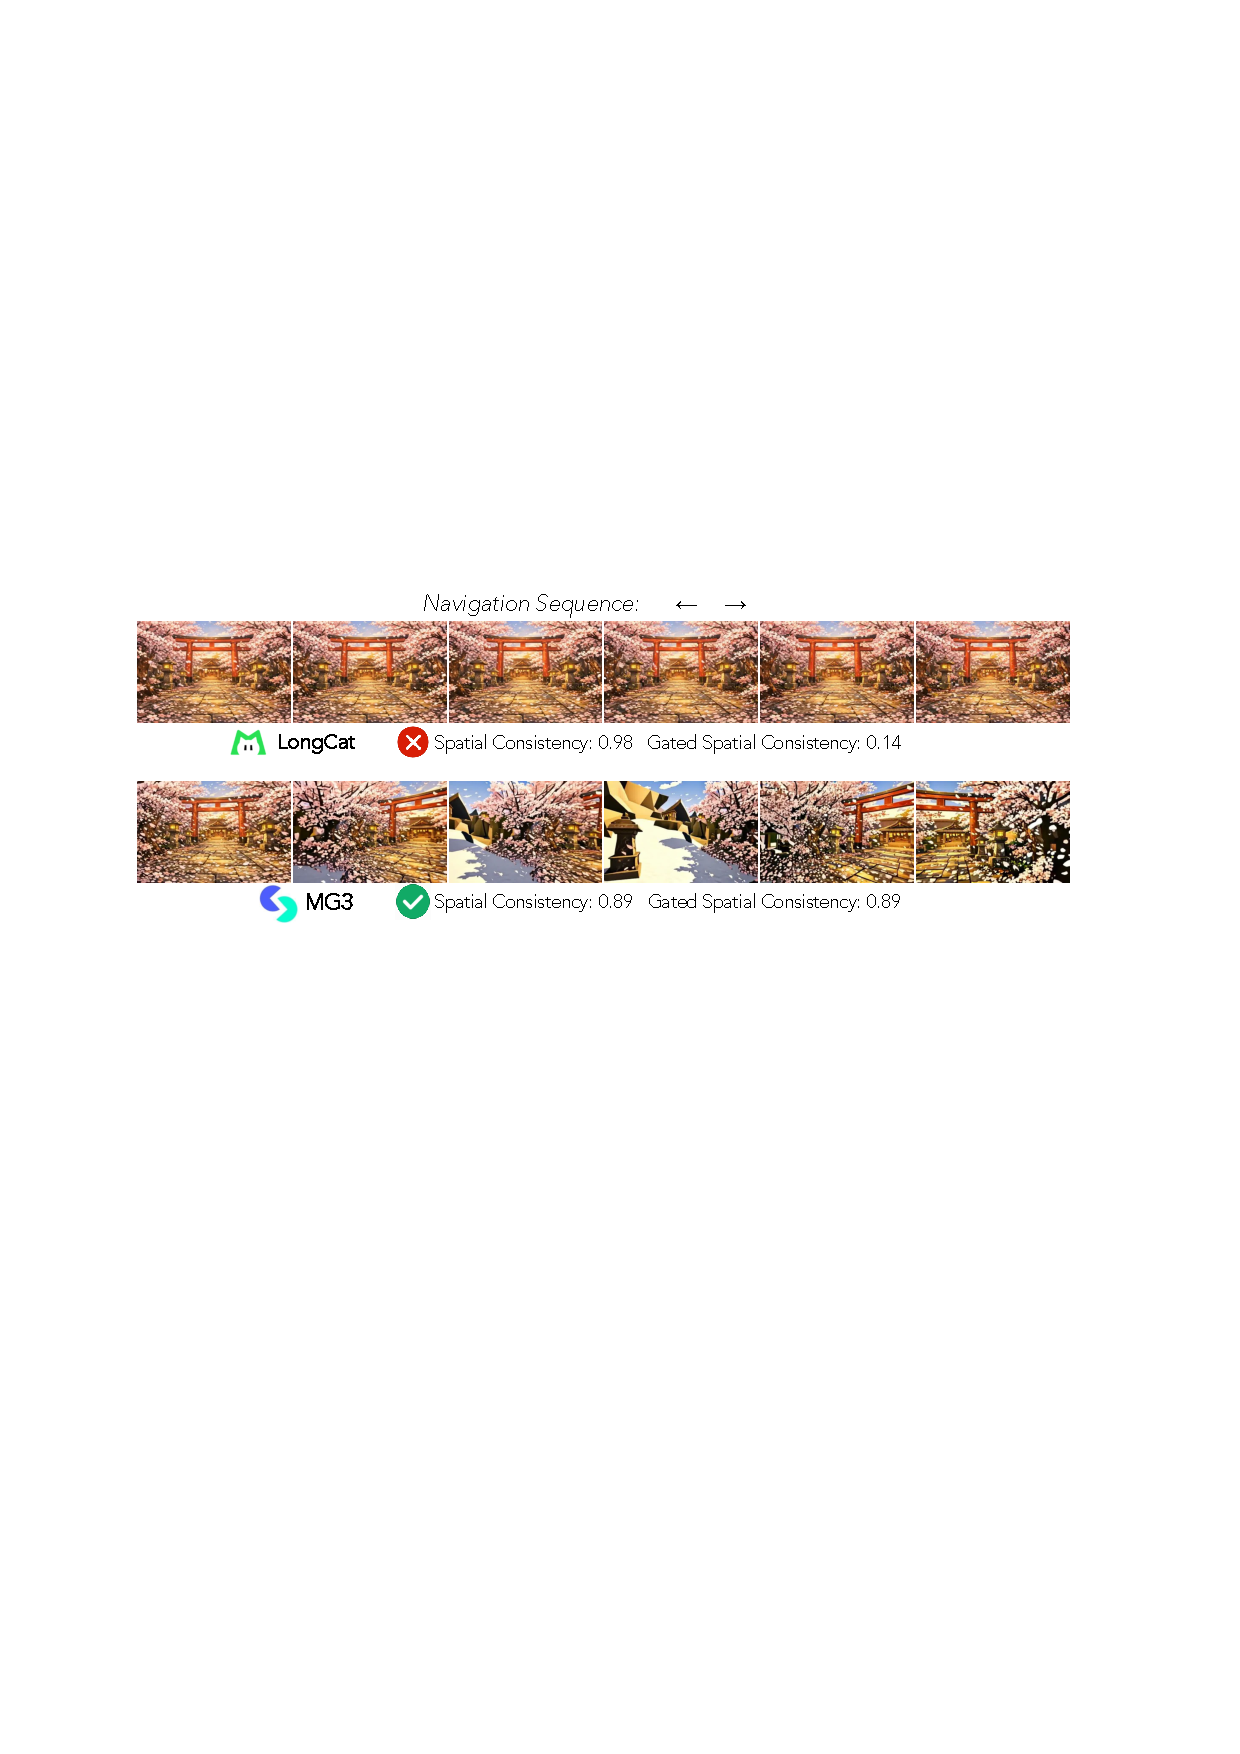
\includegraphics[width=\linewidth]{figures/spatial_cons.pdf}
\caption[Qualitative comparisons on spatial consistency]{Qualitative comparisons on spatial consistency. The gated score penalises the static scene.}
\label{fig:qual_spatial}
\end{figure}


\subsubsection{Segment Continuity}
\label{app:segment_continuity_detail}

\myparagraph{Definition.}
TransNetV2 predicts per-frame scene-boundary probabilities.
Frames exceeding a confidence threshold of $0.5$ are flagged as cut candidates, with a minimum scene length of 10 frames to suppress spurious detections.
Each video receives a binary score: $1$ if no cut is detected, $0$ otherwise.
The model-level score is the fraction of cut-free videos: $\mathrm{score} = 1 - n_{\mathrm{cut}} / N$.

\subsubsection{Perspective Consistency}
\label{app:perspective_consistency}

\myparagraph{Definition.}
For each frame where the SAM2-tracked target is present (mask area $\geq 10$\,px), we record the normalized centroid $(c_x, c_y)$ within the mask region.
Let $p = n_{\text{valid}} / n_{\text{total}}$ denote the target presence rate.
The score measures how stably the subject remains positioned across frames:
\begin{equation}
  s_{\text{centroid}} = \max\!\Bigl(0,\; 1 - \frac{\sqrt{\sigma_{c_x}^2 + \sigma_{c_y}^2}}{0.3}\Bigr) \times p,
\end{equation}
where $\sigma_{c_x}$ and $\sigma_{c_y}$ are the standard deviations of the normalized centroid coordinates over valid frames.
The presence weighting ensures that models where the target frequently disappears receive lower scores, while the threshold constant ($0.3$) is set so that moderate drift already incurs significant penalty.


\subsubsection{Reconstruction Consistency}
\label{app:reconstruction_detail}

\myparagraph{Definition.}
Depth Anything 3~\cite{lin2025depthanything3} jointly estimates per-frame depth maps and camera poses.
We evaluate 3D coherence via two complementary signals that share the same depth-based reprojection pipeline.

For a pixel $\mathbf{u}_i = (u_i, v_i, 1)^\top$ in frame $i$ with depth $d_i(\mathbf{u}_i)$, we first back-project it to 3D in camera $i$,
\begin{equation}
  \mathbf{X}_i = d_i(\mathbf{u}_i) K^{-1} \mathbf{u}_i,
\end{equation}
where $K$ is the camera intrinsic matrix.
Using the relative pose from frame $i$ to frame $j$, we transform the point into camera $j$,
\begin{equation}
  \mathbf{X}_j = R_{ji} \mathbf{X}_i + \mathbf{t}_{ji},
\end{equation}
and project it onto frame $j$,
\begin{equation}
  \hat{\mathbf{u}}_j = \pi(K \mathbf{X}_j),
\end{equation}
where $\pi([x, y, z]^\top) = (x/z, y/z)$ denotes perspective projection.

\emph{Geometric consistency} measures the reprojection displacement between the projected location $\hat{\mathbf{u}}_j$ and its matched target location $\mathbf{u}_j$ in frame $j$.
For each valid pair, we normalize the displacement by the image diagonal $D = \sqrt{H^2 + W^2}$ and compute
\begin{equation}
  e_{\mathrm{rel}}(\mathbf{u}_i) = \frac{\lVert \hat{\mathbf{u}}_j - \mathbf{u}_j \rVert_2}{D},
  \qquad
  \bar{e}_{\mathrm{rel}} = \frac{1}{N} \sum_{n=1}^{N} e_{\mathrm{rel}}(\mathbf{u}_i^{(n)}),
\end{equation}
where $N$ is the number of valid projected points.
The geometric consistency score is then
\begin{equation}
  s_{\mathrm{geo}} = \frac{1}{1 + \bar{e}_{\mathrm{rel}}}.
\end{equation}

\emph{Photometric consistency} warps the RGB value of frame $i$ to the projected location in frame $j$ using the same reprojection mapping.
Let $\hat{I}_{i \rightarrow j}$ denote the warped image and $I_j$ denote the observed frame.
We evaluate their agreement using PSNR,
\begin{equation}
  s_{\mathrm{photo}} = \mathrm{PSNR}(\hat{I}_{i \rightarrow j}, I_j)
  = 10 \log_{10} \frac{255^2}{\mathrm{MSE}(\hat{I}_{i \rightarrow j}, I_j)}.
\end{equation}

The two signals are complementary.
Geometric consistency is sensitive to structural distortion caused by incorrect depth or pose, while photometric consistency captures appearance instability such as texture flickering or color shift after geometric alignment.
Our formulation shares the reprojection-based evaluation philosophy with recent video generation alignment methods. VGGRPO~\cite{an2026vggrpo} computes a depth-space reprojection reward by comparing rendered depth maps with predicted depths to enforce cross-view geometric coherence, while VideoGPA~\cite{du2026videogpa} constructs a pixel-space reprojection signal by rendering a colored point cloud back into each view and measuring MSE and LPIPS against the original frames. In contrast, we unify both geometric and photometric evaluation within a single depth-based reprojection pipeline, using displacement error for structural fidelity and PSNR for appearance stability.
Compared with WorldScore~\cite{duan2024worldscore}, we keep both terms within the same depth-based reprojection framework.

\subsection{Physical}
\label{app:physical_detail}

The physical dimension is evaluated via two sub-metrics: causal fidelity (VLM-based) and visual plausibility (fine-tuned Qwen3VL).

\subsubsection{Causal Fidelity}
\label{app:causal_fidelity_detail}

\myparagraph{Definition.}
Causal fidelity uses \texttt{Doubao-Seed-2.0-lite} with video frames sampled at 3\,fps.
It is scored along two complementary tracks, both on a 0--3 scale. Track~1 assigns a global score for rendering-level physics and causal consistency. Track~2 averages 0--3 scores over a case-specific subset of seven physics dimensions, selected in a text-only step so that the same dimensions are evaluated across all models. When Track~2 is applicable, the per-turn score is $(s_{\text{track1}} + \bar{s}_{\text{track2}})/2$; otherwise it falls back to $s_{\text{track1}}$. The case score is the mean over all evaluated turns and lies in $[0, 3]$, and is subsequently normalised to $[0, 1]$.

\myparagraph{Prompt.} The used prompots are shown as below.

\begin{tcolorbox}[d5box, title={Causal Fidelity --- Track 1: Rendering Physics \& Causal Consistency (0--3)}]
\textbf{System:}
\begin{tcolorbox}[systemprompt]
You are evaluating the RENDERING-LEVEL visual plausibility and causal consistency of an AI-generated video segment. You will be shown a sequence of frames in temporal order.\\
\\
IMPORTANT RULES:\\
- Do NOT judge whether depicted actions are possible in the real world. Fantasy / sci-fi elements are acceptable if the setting calls for them.\\
- Do NOT penalize camera behaviour (tilting, shaking, panning, zooming, rotation). Camera motion is a cinematography choice, NOT a physics issue of the world.\\
- ONLY evaluate the physics of OBJECTS and CHARACTERS within the scene.\\
\\
Before scoring, mentally scan the frames for notable events, unexplained appearances / disappearances, and whether every visible effect has a plausible cause and every depicted action produces its expected consequences.\\
\\
Evaluate the following aspects:\\
\emph{A.~Rendering physics.} (1) solid-body integrity, (2) consistent gravity, (3) motion continuity, (4) object permanence, (5) natural deformation, (6) character physics.\\
\emph{B.~Causal consistency.} (7) no effect without cause (for non-instructed changes), (8) no cause without effect (the instructed action must produce its consequences), (9) no unrelated objects or effects appearing from nothing. The instructed action and its direct consequences are EXPECTED changes and must NOT be penalised.
\end{tcolorbox}
\vspace{4pt}
\textbf{User:}
\begin{tcolorbox}[userprompt]
Scene context: [SCENE\_DESC]\\
The instructed action for this segment is: `[ACTION]'.\\
Special physics rule: [RULE\_DESC]\\
\\
\mbox{[FRAME\_SEQUENCE]}\\
\\
First, note any notable events, state changes, or objects appearing / disappearing across the frames. Then rate the overall rendering physics AND causal consistency of this segment from 0 to 3:\\
  3 -- Good: physics and causality are natural and consistent, no significant artifacts or causal errors.\\
  2 -- Fair: noticeable problems such as some clipping, jerky motion, or 1--2 causal errors, but main actions still make sense.\\
  1 -- Poor: multiple physics violations and / or causal breakdowns, objects appear from nowhere, frequent clipping, missing consequences.\\
  0 -- Failure: physics and causality are mostly or completely broken.
\end{tcolorbox}
\end{tcolorbox}

\vspace{6pt}

\begin{tcolorbox}[d5box, title={Causal Fidelity --- Track 2: Scene-Aware Physics Dimensions (0--3, averaged)}]
\textbf{Stage 2A (dimension selection, text-only; precomputed once per case):}
\begin{tcolorbox}[systemprompt]
You are a physics evaluation assistant for AI-generated videos. Given scene context, environment details, and an action description, identify which specific physics phenomena are relevant and should be evaluated. Consider BOTH the action AND the environment, for example rain implies fluid / reflection, snow implies surface tracks, wind implies environmental forces. Select only dimensions that are clearly relevant, but do not miss obvious ones.
\end{tcolorbox}
\vspace{4pt}
\begin{tcolorbox}[userprompt]
Scene description: [SCENE\_DESCRIPTION]\\
Interaction sequence: [FULL\_INTERACTION\_SEQUENCE]\\
Environment details: [ENV\_DETAILS]\\
\\
Select ALL applicable dimensions from:\\
(1) Fluid \& Smoke: liquids, smoke, fire, steam, and underwater behaviour (buoyancy, bubbles, drifting).\\
(2) Collision \& Clipping: objects or characters physically colliding, striking, pushing, or overlapping. Do NOT select for scenes without physical contact.\\
(3) Surface Tracks \& Imprints: movement over soft, deformable surfaces (snow, sand, mud, wet ground, dust). Do NOT select for hard surfaces.\\
(4) Deformation \& Destruction: breaking, shattering, crumbling, tearing, or bending, including explosion debris.\\
(5) Wind \& Environmental Forces: wind acting on hair, cloth, leaves, particles; currents and air resistance.\\
(6) Reflection \& Lighting: water / mirror reflections, explicit point lights, directional shadows, metallic / glass reflections, or fire / lava illumination.\\
(7) Human Motion \& Expression: clearly visible human or humanoid figures whose body motion and face coherence can be judged across frames.
\end{tcolorbox}
\vspace{6pt}
\textbf{Stage 2B (shared system prompt and user template for per-dimension scoring):}
\begin{tcolorbox}[systemprompt]
You are evaluating a specific physics phenomenon in an AI-generated video segment. Score based ONLY on the specified physics dimension, not on overall video quality. These are AI-generated videos; minor rendering artifacts are acceptable. Focus on whether the specific physical behaviour is plausible.
\end{tcolorbox}
\vspace{4pt}
\begin{tcolorbox}[userprompt]
World setting: [SCENE\_DESCRIPTION]\\
\\
\mbox{[FRAME\_SEQUENCE]}\\
\\
Evaluate dimension [DIM\_ID]: [DIM\_NAME].\\
Description: [DIM\_DESCRIPTION]\\
\mbox{[DIM\_SCORING\_PROMPT]}
\end{tcolorbox}
\vspace{4pt}
The seven dimension-specific \texttt{[DIM\_SCORING\_PROMPT]} templates are reproduced verbatim below.
\end{tcolorbox}

\vspace{6pt}

\begin{tcolorbox}[d5box, title={Track 2 Rubric --- Fluid \& Smoke}]
\ttfamily\scriptsize
Rate fluid, smoke, and related effects (0--3).\\
3 = Realistic flow, splash, smoke rise, underwater drift.\\
2 = Minor artifacts but behaviour is recognisable.\\
1 = Notable issues: liquid defies gravity, smoke static, no bubbles.\\
0 = Fluid / smoke behaviour completely unrealistic or absent, or completely unrealistic.
\end{tcolorbox}

\vspace{4pt}

\begin{tcolorbox}[d5box, title={Track 2 Rubric --- Collision \& Clipping}]
\ttfamily\scriptsize
Rate collision and solid-body integrity (0--3). ONLY evaluate collisions / contacts that actually occur.\\
3 = All contacts are natural, no clipping or pass-through.\\
2 = Minor clipping but mostly plausible contacts.\\
1 = Obvious clipping: limbs pass through objects or surfaces.\\
0 = Severe clipping, objects completely ignore each other.
\end{tcolorbox}

\vspace{4pt}

\begin{tcolorbox}[d5box, title={Track 2 Rubric --- Surface Tracks \& Imprints}]
\ttfamily\scriptsize
Rate surface interaction and imprint accuracy (0--3).\\
3 = Clear, appropriate marks visible (footprints in snow, tracks in sand).\\
2 = Some marks visible but incomplete or inconsistent.\\
1 = No marks visible on a surface that should clearly show them.\\
0 = Surface shows no response at all to contact.
\end{tcolorbox}

\vspace{4pt}

\begin{tcolorbox}[d5box, title={Track 2 Rubric --- Deformation \& Destruction}]
\ttfamily\scriptsize
Rate deformation and destruction effects (0--3).\\
3 = Realistic shattering, crumbling, bending, debris scatter.\\
2 = Minor issues but deformation is recognisable.\\
1 = Deformation clearly unnatural or inconsistent.\\
0 = No deformation when expected, or completely unrealistic.
\end{tcolorbox}

\vspace{4pt}

\begin{tcolorbox}[d5box, title={Track 2 Rubric --- Wind \& Environmental Forces}]
\ttfamily\scriptsize
Rate wind and environmental force effects (0--3).\\
3 = Natural swaying, drifting, fluttering of affected objects.\\
2 = Minor issues but environmental effects are recognisable.\\
1 = Effects are stiff, static, or inconsistent with the scene.\\
0 = No environmental effects visible when expected.
\end{tcolorbox}

\vspace{4pt}

\begin{tcolorbox}[d5box, title={Track 2 Rubric --- Reflection \& Lighting}]
\ttfamily\scriptsize
Rate the accuracy of SPECIAL reflection and lighting effects (0--3). Evaluate ONLY optical effects that are actually VISIBLE in the video; do NOT penalise for effects that are absent from the scene.\\
Check for:\\
- Water / mirror reflections: do they match the shape and motion of the source?\\
- Point light sources: is the illumination range and falloff plausible?\\
- Shadows: do they point in the correct direction relative to the light?\\
- Metallic / glass surfaces: do they show plausible environment reflections?\\
\\
3 = All visible optical effects are accurate and physically consistent.\\
2 = Minor errors in one effect (e.g. reflection slightly misaligned).\\
1 = Clear errors: reflections show wrong content, shadows point wrong way, or lighting does not respond to scene changes.\\
0 = Optical effects are completely wrong or absent when clearly expected.
\end{tcolorbox}

\vspace{4pt}

\begin{tcolorbox}[d5box, title={Track 2 Rubric --- Human Motion \& Expression}]
\ttfamily\scriptsize
Rate human motion naturalness and facial expression quality (0--3). Focus on MOVEMENT ACROSS FRAMES, not just single-frame anatomy:\\
- Does the character move fluidly between poses, or jerk / teleport?\\
- Are body movements biomechanically plausible (natural gait, realistic reach, believable weight shifts)?\\
- Do limbs move in coordinated, purposeful ways, or flail randomly?\\
- Is the face coherent (no melting, distortion, or uncanny shifts)?\\
Minor structural issues (slight hand distortion, brief extra finger) should NOT heavily impact the score if overall motion is natural.\\
\\
3 = Smooth, natural human motion throughout; face is coherent.\\
2 = Mostly natural motion with minor stiffness or brief glitches.\\
1 = Clearly unnatural: jerky limbs, puppet-like movement, frozen poses, or obvious face distortion.\\
0 = Severely broken: limbs flail impossibly, body contorts unnaturally, face melts or deforms grotesquely.\\[4pt]
\rmfamily\normalsize
\textit{\small Track 2 score $\bar{s}_{\text{track2}}$ is the arithmetic mean of the 0--3 scores over all selected dimensions. Dimension selection is precomputed once per case, manually verified, and shared across all models to ensure comparability. When at least one dimension is selected, the per-turn causal fidelity score is $s = (s_{\text{track1}} + \bar{s}_{\text{track2}}) / 2$; otherwise it falls back to $s_{\text{track1}}$. The per-case score is the mean over all evaluated turns and lies in $[0, 3]$, then normalised to $[0, 1]$.}
\end{tcolorbox}

\myparagraph{Qualitative Results.}
\cref{fig:qual_pf} shows the comparison of good and bad cases, generated by different models on each sub-dimension evaluated in Track 2.

\begin{figure}[H]
\centering
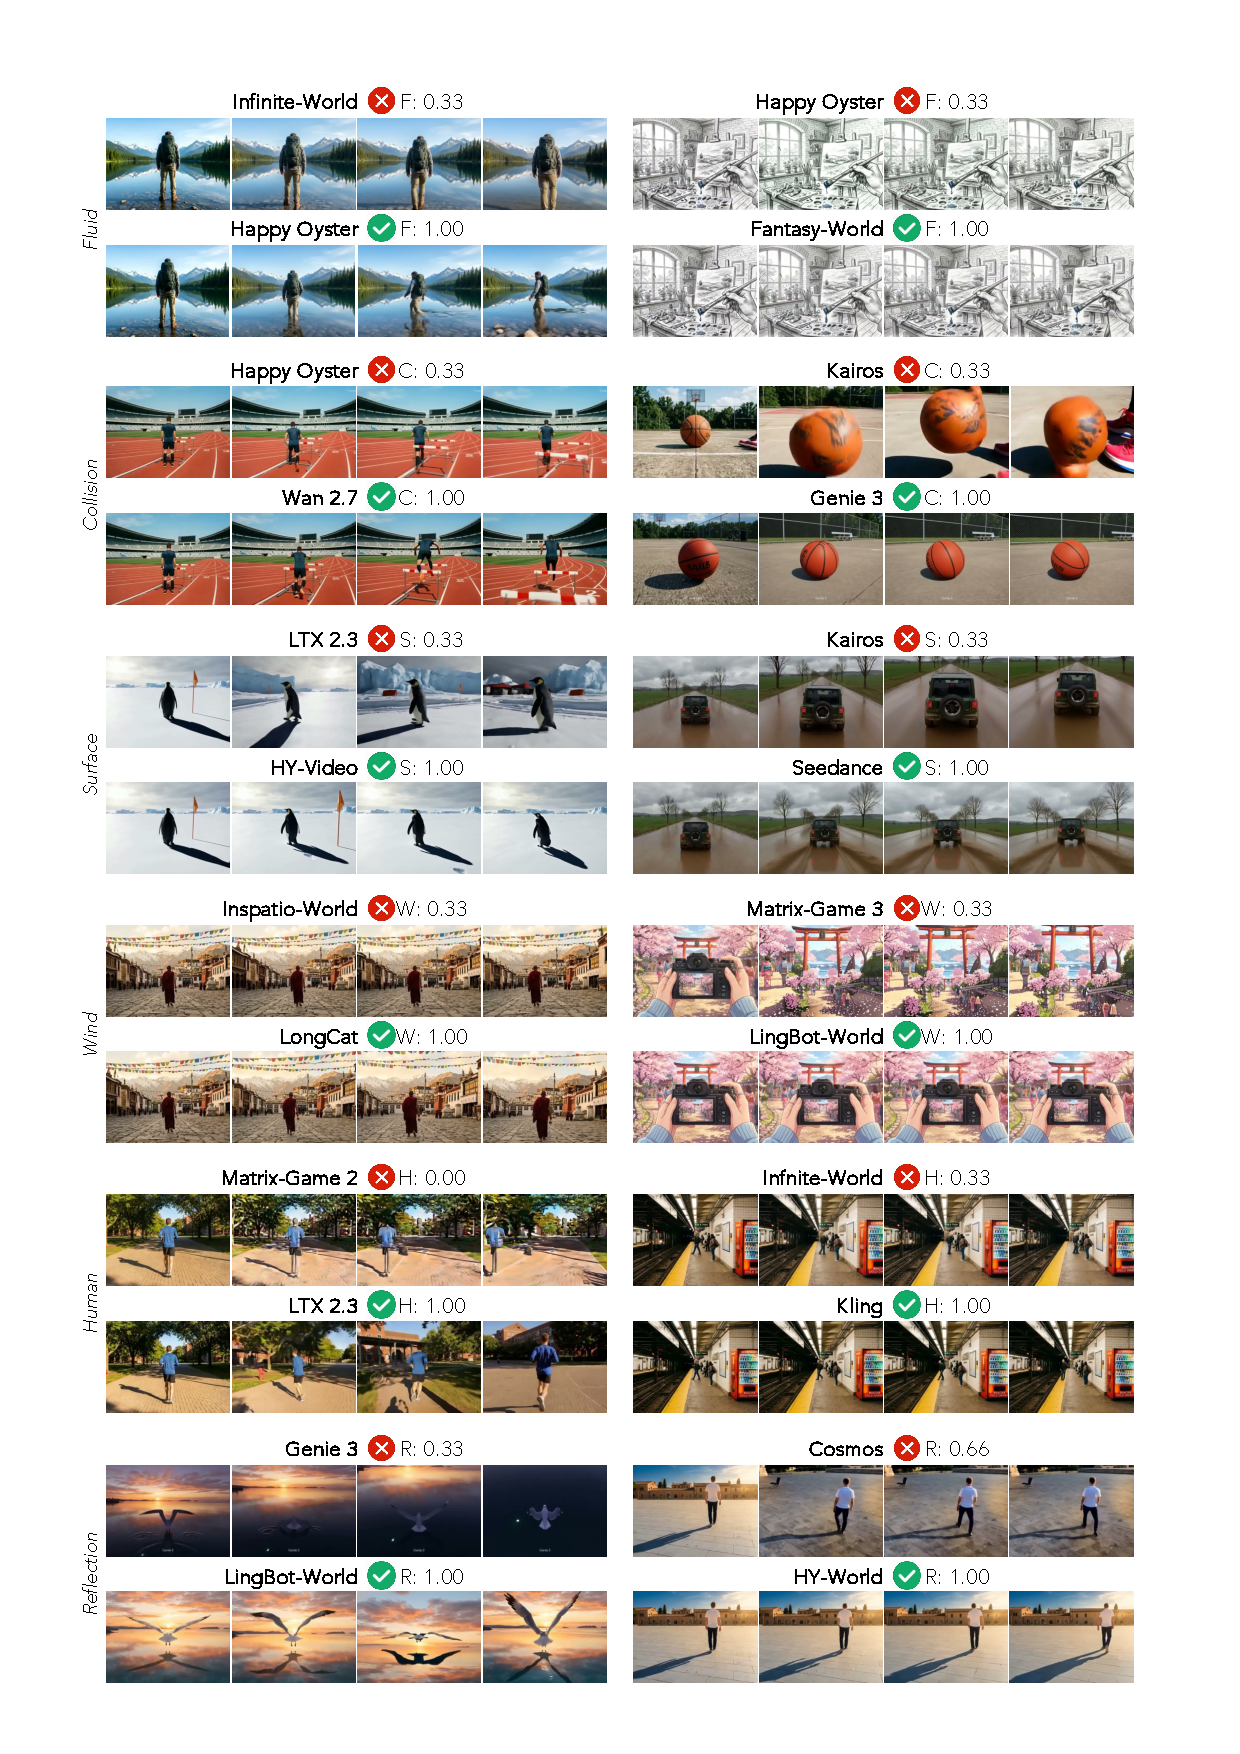
\includegraphics[width=0.88\linewidth]{figures/PF_case.orig.pdf}
\caption[Qualitative comparisons on physics compliance]{Qualitative comparisons on physics compliance.}
\label{fig:qual_pf}
\end{figure}

\myparagraph{Results.}
\cref{tab:track2_per_case_activation} lists every one of the \textbf{50} cases that receive Track 2 scoring, together with a short scene description and the seven dimension flags. A \cmark\ indicates that the dimension is included in that case's Stage 2B scoring pool, and a \xmark\ indicates that it is skipped.

\Cref{fig:radar_physics_per_dim} further decomposes Track~2 causal fidelity across the seven physics sub-dimensions. The results reveal heterogeneous failure modes across models. Reflection~\& Lighting is nearly saturated for most models, while Deformation~\& Destruction shows much larger variation despite being activated in only $4$ of the $50$ Track~2 cases, suggesting that destructive event dynamics remain challenging. Tier-wise gaps are also axis-dependent: strong models such as Wan~2.7 lead on most dimensions, but their advantage is much larger on Deformation and Human Motion than on Reflection, indicating that aggregate scores can obscure the underlying failure axes. Moreover, models with similar overall performance exhibit distinct trade-offs. Flagship text-driven systems are stronger on Fluid and Collision, LingBot-World performs best on Human Motion and Reflection but lags on Fluid and Surface, and YUME~1.5 stands out on Wind, consistent with its outdoor navigation-oriented fine-tuning. These patterns show that causal fidelity is a multi-dimensional capability, where similar overall scores may reflect qualitatively different physics profiles.


\begin{figure*}[!htbp]
  \centering
  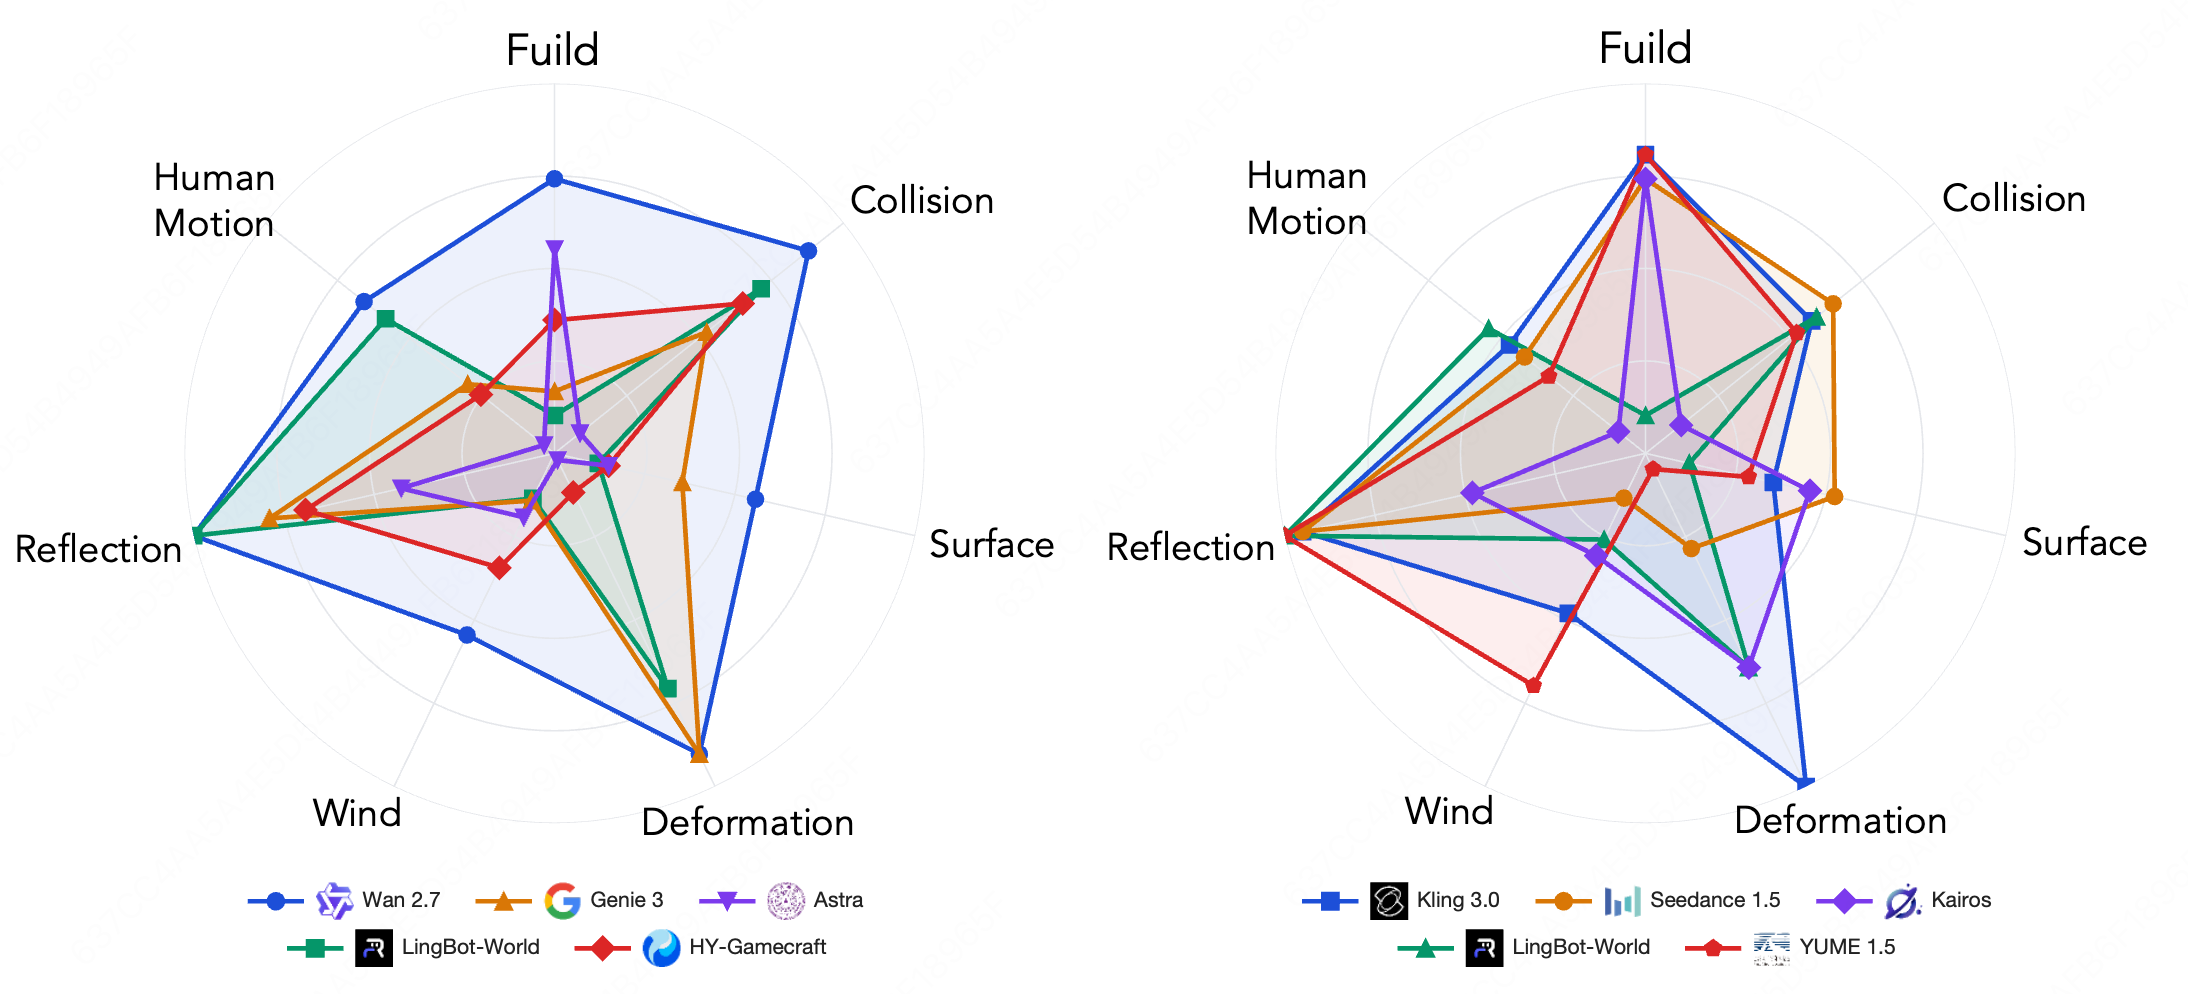
\includegraphics[width=\linewidth]{figures/PF_sub_dim.png}
  \caption[Causal Fidelity decomposed by Track 2 sub-dimensions]{Causal Fidelity decomposed along the seven Track~2 sub-dimensions. \textit{Left:} a top-to-bottom tier across paradigms. \textit{Right:} models at a similar overall tier that trade off strengths across sub-dimensions. Each axis is rescaled to its own visible range to make the per-sub-dimension differences easier to read.}
  \label{fig:radar_physics_per_dim}
\end{figure*}

\begin{table*}[!htbp]
\centering
\scriptsize
\setlength{\tabcolsep}{3pt}
\renewcommand{\arraystretch}{1.05}
\begin{tabular}{@{}l p{0.55\linewidth} ccccccc c@{}}
\toprule
\textbf{ID} & \textbf{Scene description} & \textbf{F} & \textbf{C} & \textbf{S} & \textbf{D} & \textbf{W} & \textbf{R} & \textbf{H} & \textbf{\#Dims} \\
\midrule
1   & blocky game world, Mario jumping over pipes and blocks                & \xmark & \cmark & \xmark & \xmark & \xmark & \xmark & \cmark & 2 \\
2   & foggy British street at night, handheld mockumentary view             & \xmark & \cmark & \xmark & \xmark & \xmark & \cmark & \cmark & 3 \\
3   & rainy anime city street, young woman walking amid neon                & \cmark & \cmark & \cmark & \xmark & \xmark & \cmark & \cmark & 5 \\
4   & realistic soccer pitch, player tracked in third person                & \xmark & \cmark & \xmark & \xmark & \xmark & \xmark & \cmark & 2 \\
5   & crowded anime subway interior, camera swaying with train              & \xmark & \cmark & \xmark & \xmark & \xmark & \cmark & \cmark & 3 \\
6   & living room with clothing rack, heated iron on table                  & \xmark & \cmark & \xmark & \cmark & \xmark & \cmark & \xmark & 3 \\
7   & busy urban street, dark rain cloud above pedestrians                  & \xmark & \cmark & \cmark & \xmark & \xmark & \cmark & \cmark & 4 \\
8   & sterile chemistry lab, glassware and pressure vial under lights       & \xmark & \cmark & \xmark & \xmark & \xmark & \cmark & \cmark & 3 \\
9   & Olympic red track, athlete approaching hurdles in lane                & \xmark & \cmark & \xmark & \xmark & \xmark & \xmark & \cmark & 2 \\
10  & Antarctic ice sheet, emperor penguin walking on snow                  & \xmark & \xmark & \cmark & \xmark & \cmark & \xmark & \cmark & 3 \\
11  & Tibetan monastery courtyard at golden hour, maroon-robed monk         & \xmark & \cmark & \xmark & \xmark & \cmark & \cmark & \cmark & 4 \\
12  & autumn park with fallen leaves, toddler in red running                & \xmark & \cmark & \xmark & \xmark & \cmark & \xmark & \cmark & 3 \\
13  & African savanna at sunset, elephant on dusty trail                    & \cmark & \xmark & \cmark & \xmark & \cmark & \cmark & \xmark & 4 \\
14  & white office desk, small plush keychain with green accents            & \xmark & \cmark & \xmark & \cmark & \xmark & \xmark & \xmark & 2 \\
15  & Mediterranean stone plaza, young man walking in sunlight              & \xmark & \cmark & \xmark & \xmark & \xmark & \cmark & \cmark & 3 \\
16  & mountain lake shore at dawn, hiker with green backpack                & \cmark & \cmark & \cmark & \xmark & \xmark & \cmark & \cmark & 5 \\
17  & muddy rural road after rain, dark green off-road jeep                 & \cmark & \xmark & \cmark & \xmark & \xmark & \cmark & \xmark & 3 \\
18  & African savanna trail, chestnut horse with safari rider               & \xmark & \cmark & \cmark & \xmark & \cmark & \xmark & \cmark & 4 \\
19  & misty Finnish lake at dawn, man rowing wooden boat                    & \cmark & \cmark & \xmark & \xmark & \xmark & \cmark & \cmark & 4 \\
20  & wooden beach boardwalk at golden hour, young man walking              & \cmark & \xmark & \xmark & \xmark & \cmark & \cmark & \cmark & 4 \\
21  & city park walkway, woman in red jacket walking in sun                 & \xmark & \cmark & \xmark & \xmark & \xmark & \cmark & \cmark & 3 \\
22  & seaside stone promenade, young skateboarder with board in hand        & \cmark & \cmark & \xmark & \xmark & \xmark & \cmark & \cmark & 4 \\
23  & tree-lined campus pathway, college student jogging in sun             & \xmark & \cmark & \xmark & \xmark & \xmark & \xmark & \cmark & 2 \\
24  & desert highway shoulder at sunset, backpacker walking                 & \xmark & \xmark & \cmark & \xmark & \xmark & \xmark & \cmark & 2 \\
25  & wide snowy field in winter, person on fat-tire bicycle                & \xmark & \xmark & \cmark & \xmark & \xmark & \xmark & \cmark & 2 \\
26  & hot desert midday, monitor lizard crawling on golden sand             & \xmark & \xmark & \cmark & \xmark & \xmark & \xmark & \xmark & 1 \\
27  & outdoor basketball court, orange ball bouncing on concrete            & \xmark & \cmark & \xmark & \xmark & \xmark & \cmark & \xmark & 2 \\
28  & subway platform, FPP view of vending machine by tiled wall             & \xmark & \cmark & \xmark & \xmark & \xmark & \cmark & \cmark & 3 \\
29  & cozy antique bookstore, brass globe on wooden stand                   & \xmark & \cmark & \xmark & \xmark & \xmark & \cmark & \cmark & 3 \\
30  & bustling Asian night market, red lanterns and moving crowd            & \cmark & \cmark & \xmark & \xmark & \xmark & \cmark & \cmark & 4 \\
31  & science classroom interior, human skeleton model near blackboard      & \xmark & \cmark & \xmark & \xmark & \xmark & \cmark & \cmark & 3 \\
32  & coastal city aerial view, FPP seabird flight with beak                 & \cmark & \cmark & \xmark & \xmark & \xmark & \xmark & \xmark & 2 \\
33  & abandoned warehouse, racing quadcopter flying between pillars         & \xmark & \cmark & \xmark & \xmark & \xmark & \cmark & \xmark & 2 \\
34  & countryside farmland, colorful hot air balloon rising                 & \xmark & \xmark & \xmark & \xmark & \xmark & \xmark & \cmark & 1 \\
35  & calm ocean at sunset, white seagull diving above water                & \cmark & \xmark & \xmark & \xmark & \xmark & \cmark & \xmark & 2 \\
36  & supermarket aisle, tall shelves with stacked red cans                 & \xmark & \cmark & \xmark & \xmark & \xmark & \cmark & \cmark & 3 \\
37  & cherry blossom garden in spring, viewer with camera viewfinder        & \xmark & \cmark & \xmark & \xmark & \cmark & \xmark & \cmark & 3 \\
38  & war-torn city ruins, FPP view holding military grenade                 & \cmark & \cmark & \xmark & \cmark & \cmark & \xmark & \cmark & 5 \\
39  & misty lakeside at dawn, viewer holding bamboo fishing rod             & \cmark & \cmark & \xmark & \xmark & \xmark & \cmark & \cmark & 4 \\
40  & sunlit artist studio, viewer holding paintbrush near canvas           & \xmark & \cmark & \xmark & \xmark & \xmark & \cmark & \cmark & 3 \\
41  & snowy tundra under aurora borealis, green purple lights               & \xmark & \cmark & \cmark & \xmark & \xmark & \cmark & \xmark & 3 \\
42  & floating sky island anime, fairy girl with dragonfly wings            & \cmark & \xmark & \xmark & \xmark & \cmark & \cmark & \cmark & 4 \\
43  & lavender field at golden hour, woman in white, oil-painting style     & \xmark & \xmark & \cmark & \xmark & \cmark & \cmark & \cmark & 4 \\
44  & magical toy workshop, wooden puppet walking among stations            & \xmark & \cmark & \xmark & \xmark & \xmark & \cmark & \cmark & 3 \\
45  & underwater ancient ruins (CG), mermaid among marble columns           & \cmark & \cmark & \cmark & \xmark & \xmark & \cmark & \cmark & 5 \\
46  & moonlit rooftops, ink-wash ninja running across tiles                 & \xmark & \cmark & \xmark & \xmark & \xmark & \xmark & \cmark & 2 \\
47  & Middle Eastern bazaar (flat), fruit merchant pushing cart             & \xmark & \cmark & \xmark & \xmark & \xmark & \xmark & \cmark & 2 \\
48  & surreal melting landscape, brass robot among dripping clocks          & \xmark & \cmark & \cmark & \cmark & \xmark & \xmark & \cmark & 4 \\
49  & spooky haunted garden, glowing ghost dog among jack-o-lanterns        & \xmark & \cmark & \xmark & \xmark & \xmark & \cmark & \xmark & 2 \\
50  & volcanic crater edge (CG), dragon hatchling flying along rim          & \cmark & \xmark & \xmark & \xmark & \cmark & \cmark & \cmark & 4 \\
\midrule
\textbf{Total} & \textbf{(50 cases)} & 15 & 38 & 14 & 4 & 11 & 32 & 39 & 153 \\
\bottomrule
\end{tabular}
\caption[Per-case Track 2 dimension activation]{Per-case Track 2 dimension activation for all \textbf{50} cases that receive Track 2 scoring. Columns: F~= Fluid~\& Smoke, C~= Collision~\& Clipping, S~= Surface Tracks, D~= Deformation~\& Destruction, W~= Wind~\& Environmental Forces, R~= Reflection~\& Lighting, H~= Human Motion~\& Expression. The final row aggregates the activation count of each dimension over all 50 cases, summing to 153 dimension-case pairs (mean $\approx 3.06$ dimensions per case).}
\label{tab:track2_per_case_activation}
\end{table*}

\subsubsection{Visual Plausibility}
\label{app:visual_plausibility_detail}

\myparagraph{Definition.}
Visual plausibility measures whether a generated video is visually realistic and physically reasonable. It focuses on the overall appearance quality, temporal consistency, object structure, motion coherence, and whether the depicted dynamics conform to common-sense physical principles. We evaluate visual plausibility using a fine-tuned Qwen3-VL-30B-A3B model.

\myparagraph{Prompt.}
All videos are evaluated with a fixed prompt. The input video is sampled at 2 FPS, and the maximum number of pixels per frame is set to 602,112. The prompt used for both training and inference is shown below.

\begin{tcolorbox}[d5box, title={Visual Plausibility --- Fine-tuned Qwen3-VL-30B-A3B}]
\ttfamily\scriptsize
Suppose you are an expert in judging and evaluating the quality of AI-generated videos, please watch the above provided video and give scores for the video's truthfulness and rationality, i.e., whether the video's overall appearance and motion are consistent with our common-sense and physical principles.\\
\\
Your rating should be chosen from the following five categories: Perfect, Good, Fair, Poor, and Bad. Now please rate this video:
\end{tcolorbox}

\myparagraph{Training Data.}
To train the visual plausibility scorer, we construct an internal annotation set consisting of approximately 6K videos generated by multiple closed-source and open-source image-to-video models. The videos cover diverse subjects, scenes, visual styles, camera motions, and interaction patterns. Internal expert annotators are first trained with unified rating guidelines, and then each video is independently rated by three annotators on a 1--5 scale, where 5 denotes the highest visual plausibility and 1 denotes the lowest. The final ground-truth score of each video is computed as the average of the three annotator scores.

\myparagraph{Score Prediction and Optimization.}
We conduct full-parameter fine-tuning upon the pre-trained Qwen3-VL-30B-A3B checkpoint~\footnote{\url{https://huggingface.co/Qwen/Qwen3-VL-30B-A3B-Instruct.}} to regress the human-annotated visual plausibility score. Given a video and the above prompt, we extract the next-token prediction distribution at the final prompt token. Let the five rating tokens be
\(\{\texttt{Perfect}, \texttt{Good}, \texttt{Fair}, \texttt{Poor}, \texttt{Bad}\}\),
corresponding to scores \(\{5,4,3,2,1\}\), respectively. We take the model probabilities assigned to these five tokens and renormalize them over the rating set:
\[
\tilde{p}_c =
\frac{p_c}{\sum_{c' \in \mathcal{C}} p_{c'}},
\quad
\mathcal{C}=\{\texttt{Perfect}, \texttt{Good}, \texttt{Fair}, \texttt{Poor}, \texttt{Bad}\}.
\]
The predicted visual plausibility score is then computed as the expectation over the five ordered categories:
\[
\hat{s}
=
5\tilde{p}_{\texttt{Perfect}}
+4\tilde{p}_{\texttt{Good}}
+3\tilde{p}_{\texttt{Fair}}
+2\tilde{p}_{\texttt{Poor}}
+1\tilde{p}_{\texttt{Bad}}.
\]
Given the ground-truth human score \(s\), the model is optimized with mean squared error:
\[
\mathcal{L}_{\mathrm{VP}} = (\hat{s} - s)^2.
\]
This formulation preserves the ordinal structure of the five rating categories while allowing the model to produce a continuous visual plausibility score aligned with averaged human judgments. The trained model achieves a Pearson Linear Correlation Coefficient~(PLCC) of 0.92 against ground-truth label, demonstrating strong human preference alignment.
